\documentclass[11pt,letterpaper]{article}
% PDF reproductible : sans date de compilation ni identifiant aleatoire, pour que git ne voie pas
% de changement quand le contenu est le meme
\pdfinfoomitdate=1
\pdftrailerid{}
\pdfsuppressptexinfo=-1

% Pour les figures et les schémas
\usepackage{float}
\usepackage{tikz}
\usetikzlibrary{arrows.meta, positioning}
\usepackage{graphicx,caption,subcaption}
\graphicspath{{./}}
\usepackage{enumitem}
\setlist[itemize]{label=\textbullet}
\usepackage{booktabs, array}
\usepackage{xcolor}

% Packages pour écrire en français
\usepackage[french]{babel}
\usepackage[utf8]{inputenc}
\usepackage[T1]{fontenc}
\addto\captionsfrench{\renewcommand{\tablename}{Tableau}}

% Maths et navigation dans le pdf
\usepackage{amsmath, amssymb}
\usepackage{hyperref}
\hypersetup{
    pdftitle={Contrôle non destructif des matériaux: Utilisation du Topaz (ultrasons phase array)},
    pdfauthor={Louis-Félix Brodeur, Simon Larouche-Tremblay}
}

% Marges, police de caractère et pied de page
\usepackage{geometry}
\geometry{top=23mm, bottom=23mm, left=20mm, right=20mm}
\usepackage{cochineal}
\usepackage{fancyhdr}
\pagestyle{fancy}
\fancyhf{}
\renewcommand{\headrulewidth}{0pt}
\setlength{\headheight}{13.6pt}
\cfoot{\small GPH-3000 TRAVAUX PRATIQUES AVANC\'ES \qquad Page \thepage}

\parindent=0mm % pas d'indentation

% Encadré pour une mise en garde
\newcommand{\attention}[1]{%
  \begin{center}
  \fbox{\begin{minipage}{0.92\linewidth}
  \textbf{Attention}\\[1mm]
  #1
  \end{minipage}}
  \end{center}
}

\begin{document}
\shorthandoff{;:!?}

\begin{center}
{\Large Contr\^ole non destructif des mat\'eriaux}\\[2mm]
{\huge Utilisation du Topaz (ultrasons phase array)}\\[6mm]
{\sc GPH-3000}\\
{\sc Louis-F\'elix Brodeur, Simon Larouche-Tremblay}\\
{\sc Septembre 2026}
\end{center}

\begin{center}
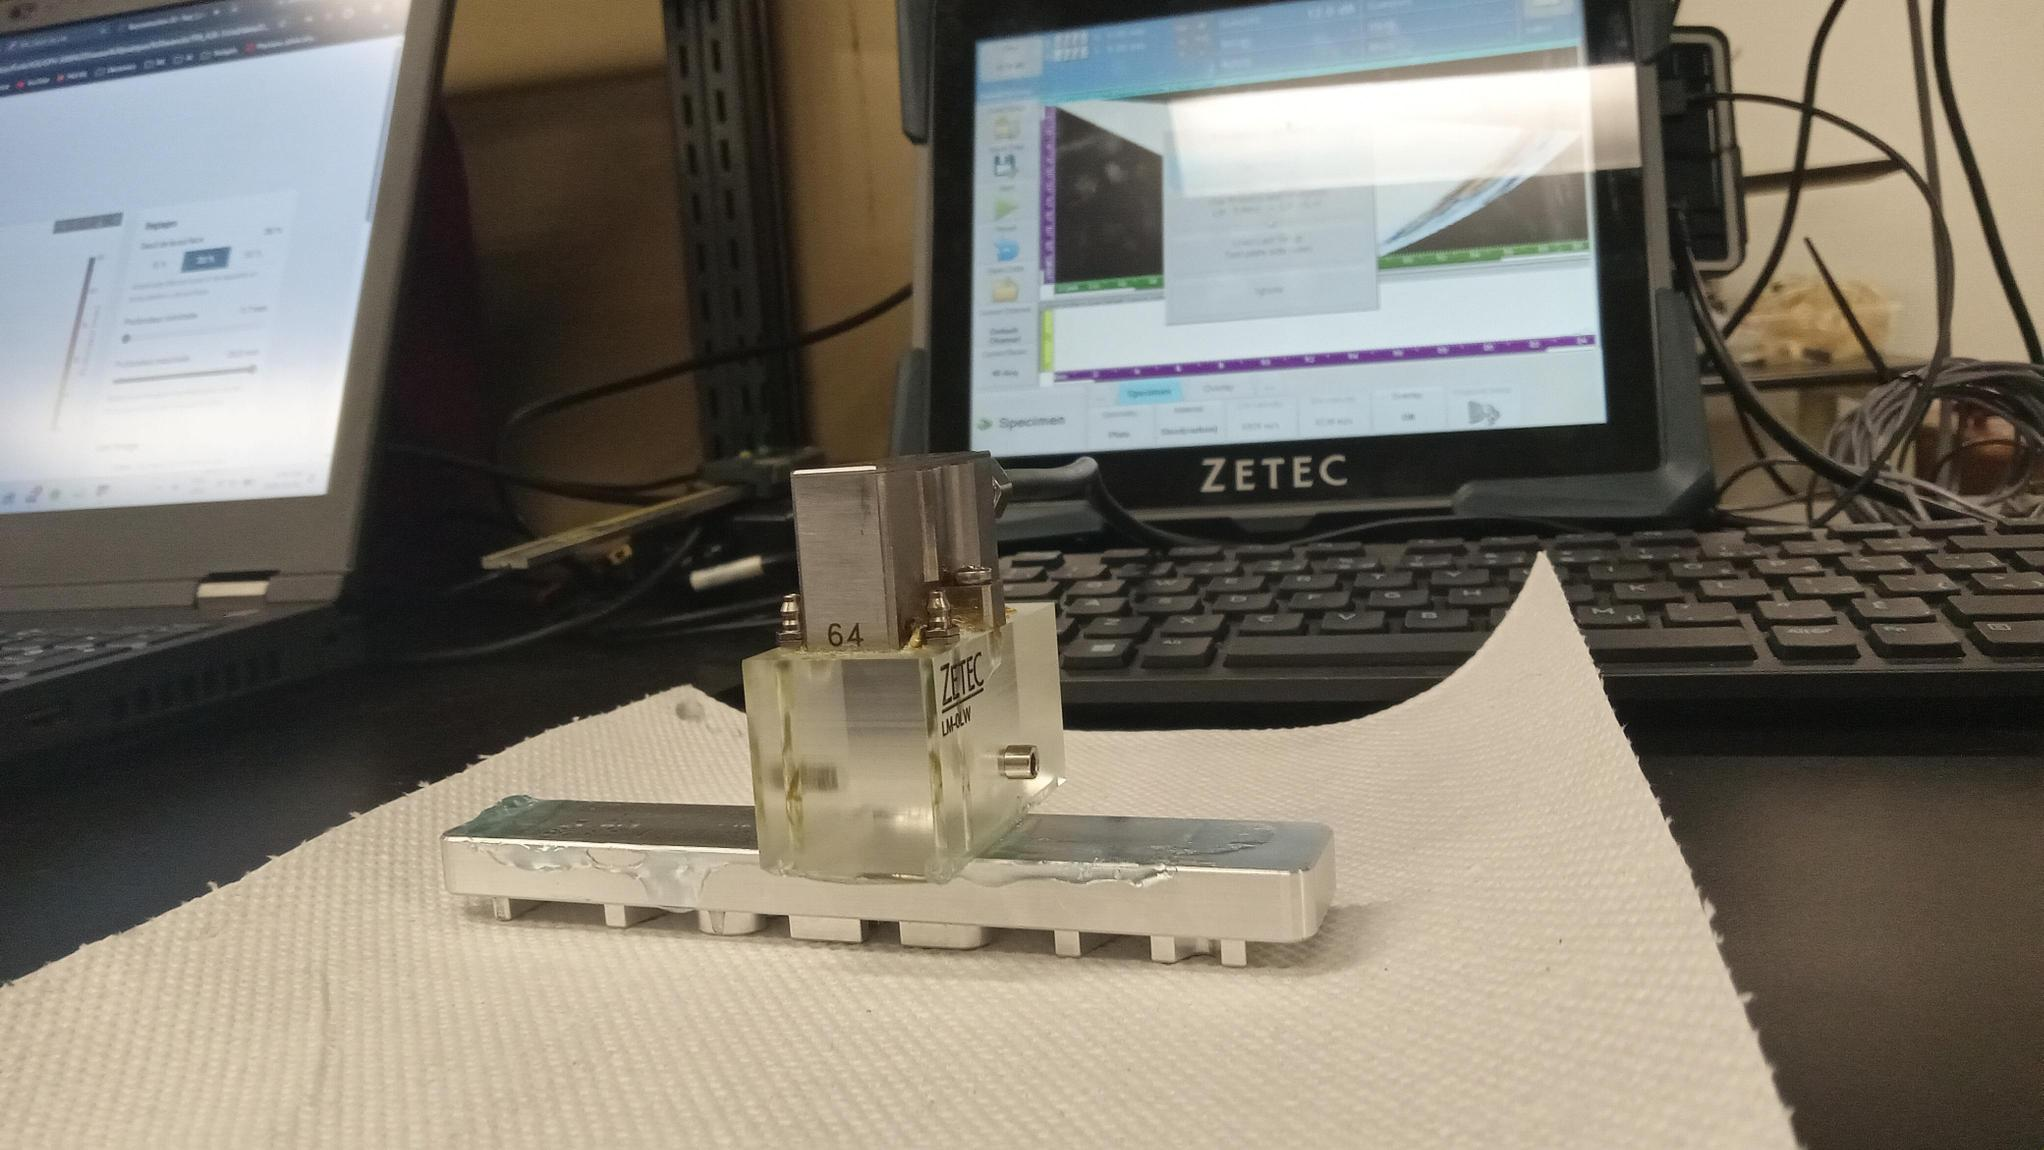
\includegraphics[width=9cm]{../../figures/Photos_Lab/PageTitreProtocole3.jpg}
\end{center}

\vspace{4mm}

\section{Principe du phase array}
\label{sec:theorie}

Une sonde \`a ultrasons conventionnelle, comme celle utilis\'ee dans le document Ultrasons, contient un seul \'el\'ement pi\'ezo\'electrique. Cet \'el\'ement \'emet un faisceau dont la direction est fix\'ee par la g\'eom\'etrie de la sonde et ne peut \^etre chang\'ee qu'en la d\'epla\c cant physiquement.

Une sonde phase array contient plusieurs \'el\'ements pi\'ezo\'electriques ind\'ependants, align\'es en r\'eseau. Chaque \'el\'ement peut \^etre excit\'e s\'epar\'ement, avec un d\'elai qui lui est propre. Si tous les \'el\'ements sont excit\'es en m\^eme temps, leurs ondes s'additionnent comme si un seul \'el\'ement avait \'et\'e utilis\'e. Mais si l'excitation de chaque \'el\'ement est retard\'ee d'une quantit\'e pr\'ecise par rapport \`a ses voisins, les fronts d'onde \'emis par chaque \'el\'ement ne sont plus en phase au moment de leur \'emission. Ils peuvent alors interf\'erer de fa\c con constructive dans une direction diff\'erente de la normale \`a la sonde, ou converger vers un point de focalisation \`a une profondeur donn\'ee. L'ensemble de ces d\'elais s'appelle une loi focale. C'est ce principe qui permet de diriger et de focaliser \'electroniquement le faisceau, sans d\'eplacer la sonde.

\begin{figure}[H]
\centering
\begin{tikzpicture}[scale=1]
  \foreach \i in {0,...,6} {
    \draw[fill=gray!30] (\i*0.7,0) rectangle ++(0.5,0.3);
  }
  % Délais proportionnels à (d_max - d_i), d_i = distance de l'élément i au point focal F
  \foreach \i/\h in {0/0.15,1/0.56,2/0.90,3/1.17,4/1.33,5/1.36,6/1.27} {
    \draw[-{Latex[length=2mm]}, thick] (\i*0.7+0.25,0.3) -- ++(0,\h);
  }
  \draw[dashed, gray] plot[smooth] coordinates {(0.25,0.45) (0.95,0.86) (1.65,1.20) (2.35,1.47) (3.05,1.63) (3.75,1.66) (4.45,1.57)};
  \coordinate (F) at (3.6,-3.2);
  \foreach \i in {0,...,6} {
    \draw[blue, thick] (\i*0.7+0.25,0) -- (F);
  }
  \fill (F) circle (2pt);
  \node[below] at (F) {Point focal};
  \node[left] at (-0.3,0.7) {D\'elais};
  \node[left] at (-0.3,-1.5) {Faisceaux};
\end{tikzpicture}
\caption{D\'elais d'excitation des \'el\'ements (fl\`eches noires) pour focaliser le faisceau en un point focal. L'\'el\'ement le plus loin du point focal est excit\'e en premier, et le plus proche en dernier.}
\label{fig:loi-focale}
\end{figure}

Le logiciel UltraVision Touch permet de combiner plusieurs lois focales pour balayer une pi\`ece de deux fa\c cons diff\'erentes. Dans un balayage sectoriel, l'angle de r\'efraction du faisceau varie d'une loi focale \`a l'autre alors que le groupe d'\'el\'ements utilis\'e, appel\'e l'ouverture, reste le m\^eme: ceci demande normalement un sabot \`a angle, taill\'e pour permettre plusieurs angles de r\'efraction utiles. Dans un balayage lin\'eaire, c'est plut\^ot l'ouverture active qui se d\'eplace \'electroniquement le long du r\'eseau, \`a angle de r\'efraction constant. Ce deuxi\`eme mode revient \`a d\'eplacer une sonde conventionnelle le long d'une pi\`ece, mais sans aucun mouvement m\'ecanique.

\begin{figure}[H]
\centering
\begin{tikzpicture}[scale=1]
  \foreach \i in {0,...,15} {
    \draw (\i*0.4,0) rectangle ++(0.3,0.3);
  }
  \foreach \i in {1,...,4} {
    \draw[fill=blue!30] (\i*0.4,0) rectangle ++(0.3,0.3);
  }
  \draw[blue, thick, -{Latex[length=2mm]}] (2.5*0.4+0.15,0) -- ++(0,-1.2);
  \foreach \i in {6,...,9} {
    \draw[fill=orange!40] (\i*0.4,0) rectangle ++(0.3,0.3);
  }
  \draw[orange!80!black, thick, -{Latex[length=2mm]}] (7.5*0.4+0.15,0) -- ++(0,-1.2);
  \foreach \i in {11,...,14} {
    \draw[fill=green!30] (\i*0.4,0) rectangle ++(0.3,0.3);
  }
  \draw[green!50!black, thick, -{Latex[length=2mm]}] (12.5*0.4+0.15,0) -- ++(0,-1.2);
  \node[below] at (2.5*0.4+0.15,-1.2) {\small 1};
  \node[below] at (7.5*0.4+0.15,-1.2) {\small 2};
  \node[below] at (12.5*0.4+0.15,-1.2) {\small 3};
\end{tikzpicture}
\caption{Trois positions de l'ouverture active (en couleur) lors d'un balayage lin\'eaire \`a 0\textdegree. Au laboratoire, l'ouverture avance d'un seul \'el\'ement entre deux faisceaux.}
\label{fig:e-scan}
\end{figure}

Le sabot disponible pour ce laboratoire est un sabot droit, adapt\'e \`a une onde longitudinale \`a incidence normale. C'est donc le balayage lin\'eaire, illustr\'e \`a la Figure~\ref{fig:e-scan}, qui est utilis\'e dans les manipulations d\'ecrites \`a la Section~\ref{sec:manipulations}.

\section{Fonctionnement du Topaz}

\subsection{Pr\'esentation de l'appareil}

Le Topaz est un appareil portable qui int\`egre le pulseur-r\'ecepteur, l'\'electronique de traitement et un \'ecran tactile permettant de faire fonctionner UltraVision Touch directement sur l'appareil, sans ordinateur externe (Figure~\ref{fig:interface}). Il peut \^etre aliment\'e par une batterie amovible ou directement au 120~V. Le matériel utilisé pour ce guide est donné au Tableau~\ref{tab:materiel}.

\begin{table}[H]
\centering
\caption{Mat\'eriel utilis\'e pour ce guide.}
\label{tab:materiel}
\small
\begin{tabular}{p{5.6cm}llp{1.7cm}}
\toprule
\'El\'ement & Num\'ero de pi\`ece & Mod\`ele & N\textsuperscript{o} de s\'erie \\
\midrule
Topaz16 (configuration 16/128) & 10053725 & ZPA-IUT-TOPAZ-16/128P-KIT & 705745 \\
Sonde lin\'eaire LM 5~MHz, 64 \'el\'ements & 10039141 & ZPA-PB1D-LM-5MHZ-REX-5M-ZPAC & B1234003 \\
Sabot droit LM-0LW & 10038863 & ZPA-ACC-W-LM-OLW-IH-FL & non indiqu\'e \\
Mini-encodeur & 10040557 & ZGN-ACC-ZPAC-ENC-5M-DE15 & 706440 \\
\bottomrule
\end{tabular}
\end{table}

Le panneau lat\'eral droit regroupe les connecteurs: un connecteur d\'edi\'e \`a la sonde phase array, verrouill\'e par un loquet, ainsi que des connecteurs conventionnels non utilis\'es dans ce document.

\begin{figure}[H]
\centering
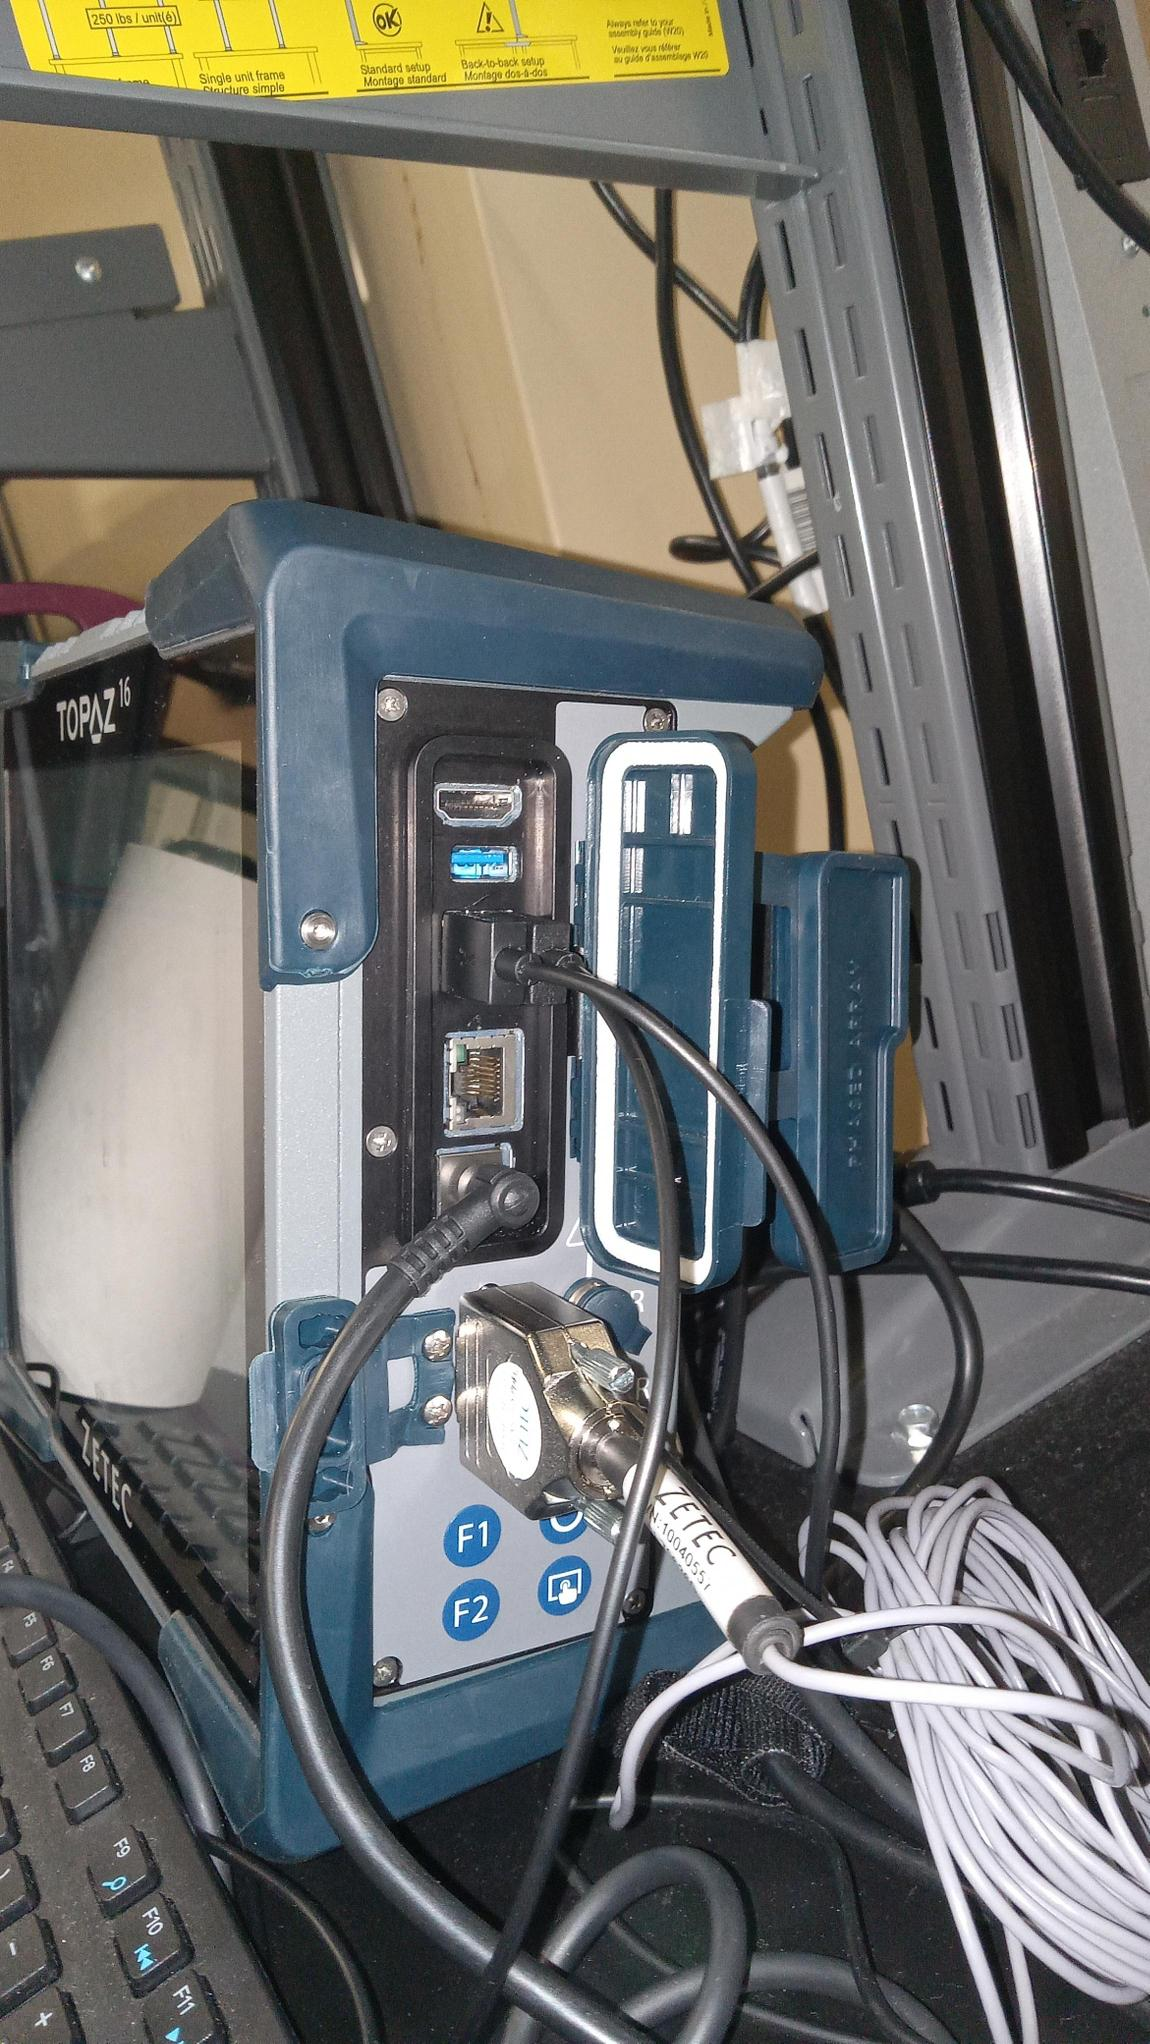
\includegraphics[height=9cm]{../../figures/Photos_Lab/TopazCoteDroit.jpg}
\caption{Panneau lat\'eral droit du Topaz.}
\label{fig:panneau-lateral}
\end{figure}

\subsection{Mise sous tension}

Avant de mettre le Topaz sous tension, v\'erifier qu'une batterie charg\'ee est install\'ee ou brancher le cordon d'alimentation. Appuyer ensuite sur le bouton marche/arr\^et: le voyant d'alimentation s'allume en vert et la s\'equence de d\'emarrage s'amorce. Il est recommand\'e de laisser l'appareil se stabiliser une dizaine de minutes avant de commencer les mesures.

\subsection{D\'epannage au d\'emarrage}
\label{sec:depannage}

Le Topaz passe par le BIOS au d\'emarrage. La proc\'edure suivante est \`a suivre \`a chaque mise sous tension, avec un clavier USB branch\'e au Topaz. Les \'ecrans sont montr\'es \`a la Figure~\ref{fig:bios}.

\begin{enumerate}
  \item \`A l'allumage, un \'ecran de d\'emarrage appara\^it pendant environ 1~seconde (Figure~\ref{fig:bios-demarrage}). Pendant cet \'ecran, appuyer sur Suppr (Del) ou \'Echap (Esc) sur le clavier pour entrer dans le BIOS.
  \item Une fen\^etre Enter Password appara\^it (Figure~\ref{fig:bios-mdp}). Il n'y a pas de mot de passe: appuyer simplement sur Enter.
  \item Dans le BIOS (Figure~\ref{fig:bios-page}), choisir Save and Exit et confirmer avec Enter. Le Topaz d\'emarre alors normalement dans UltraVision Touch.
  \item UltraVision Touch propose de choisir la sonde: prendre la LM de 5~MHz et le sabot LM-0LW, puis charger la configuration (Section~\ref{sec:configuration}).
\end{enumerate}

Les probl\`emes suivants sont connus pour la version 3.8R11 du logiciel.

\begin{enumerate}
  \item Ne pas brancher de splitter pendant le d\'emarrage. Si une fen\^etre propose une mise \`a jour FPGA, la refuser. L'accepter emp\^eche la connexion \`a UltraVision et oblige \`a r\'einstaller le logiciel (anomalie B1833 du document \og Limitations and Remaining Anomalies \fg{} de la version 3.8R11).
  \item Les boutons F1 et F2 du TOPAZ16 ne fonctionnent pas en version 3.8R11 (anomalie B2060).
\end{enumerate}

\begin{figure}[H]
\centering
\begin{subfigure}[t]{0.32\textwidth}
  \centering
  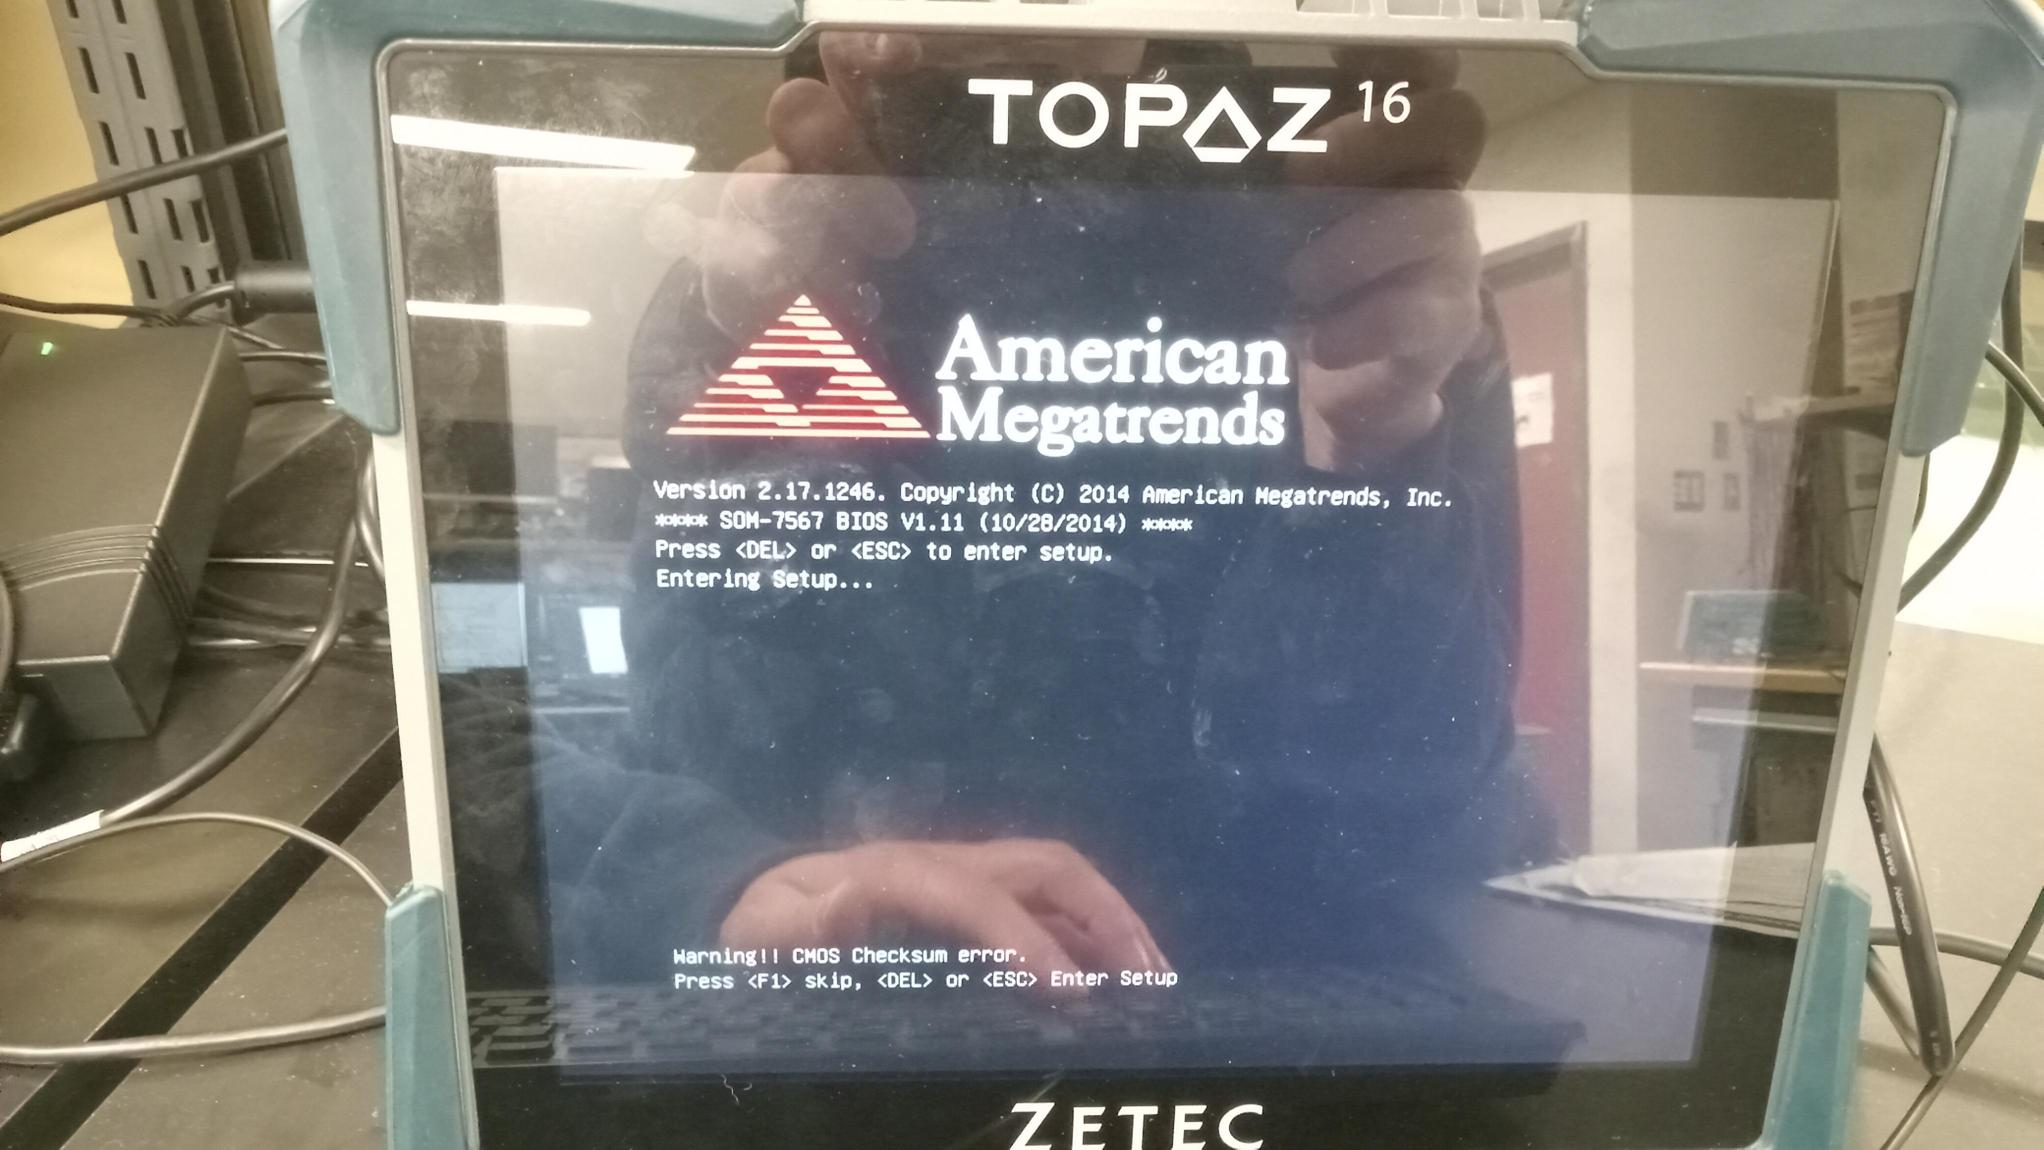
\includegraphics[width=\textwidth]{../../figures/Photos_Lab/EnterBios1.jpg}
  \caption{}
  \label{fig:bios-demarrage}
\end{subfigure}
\hfill
\begin{subfigure}[t]{0.32\textwidth}
  \centering
  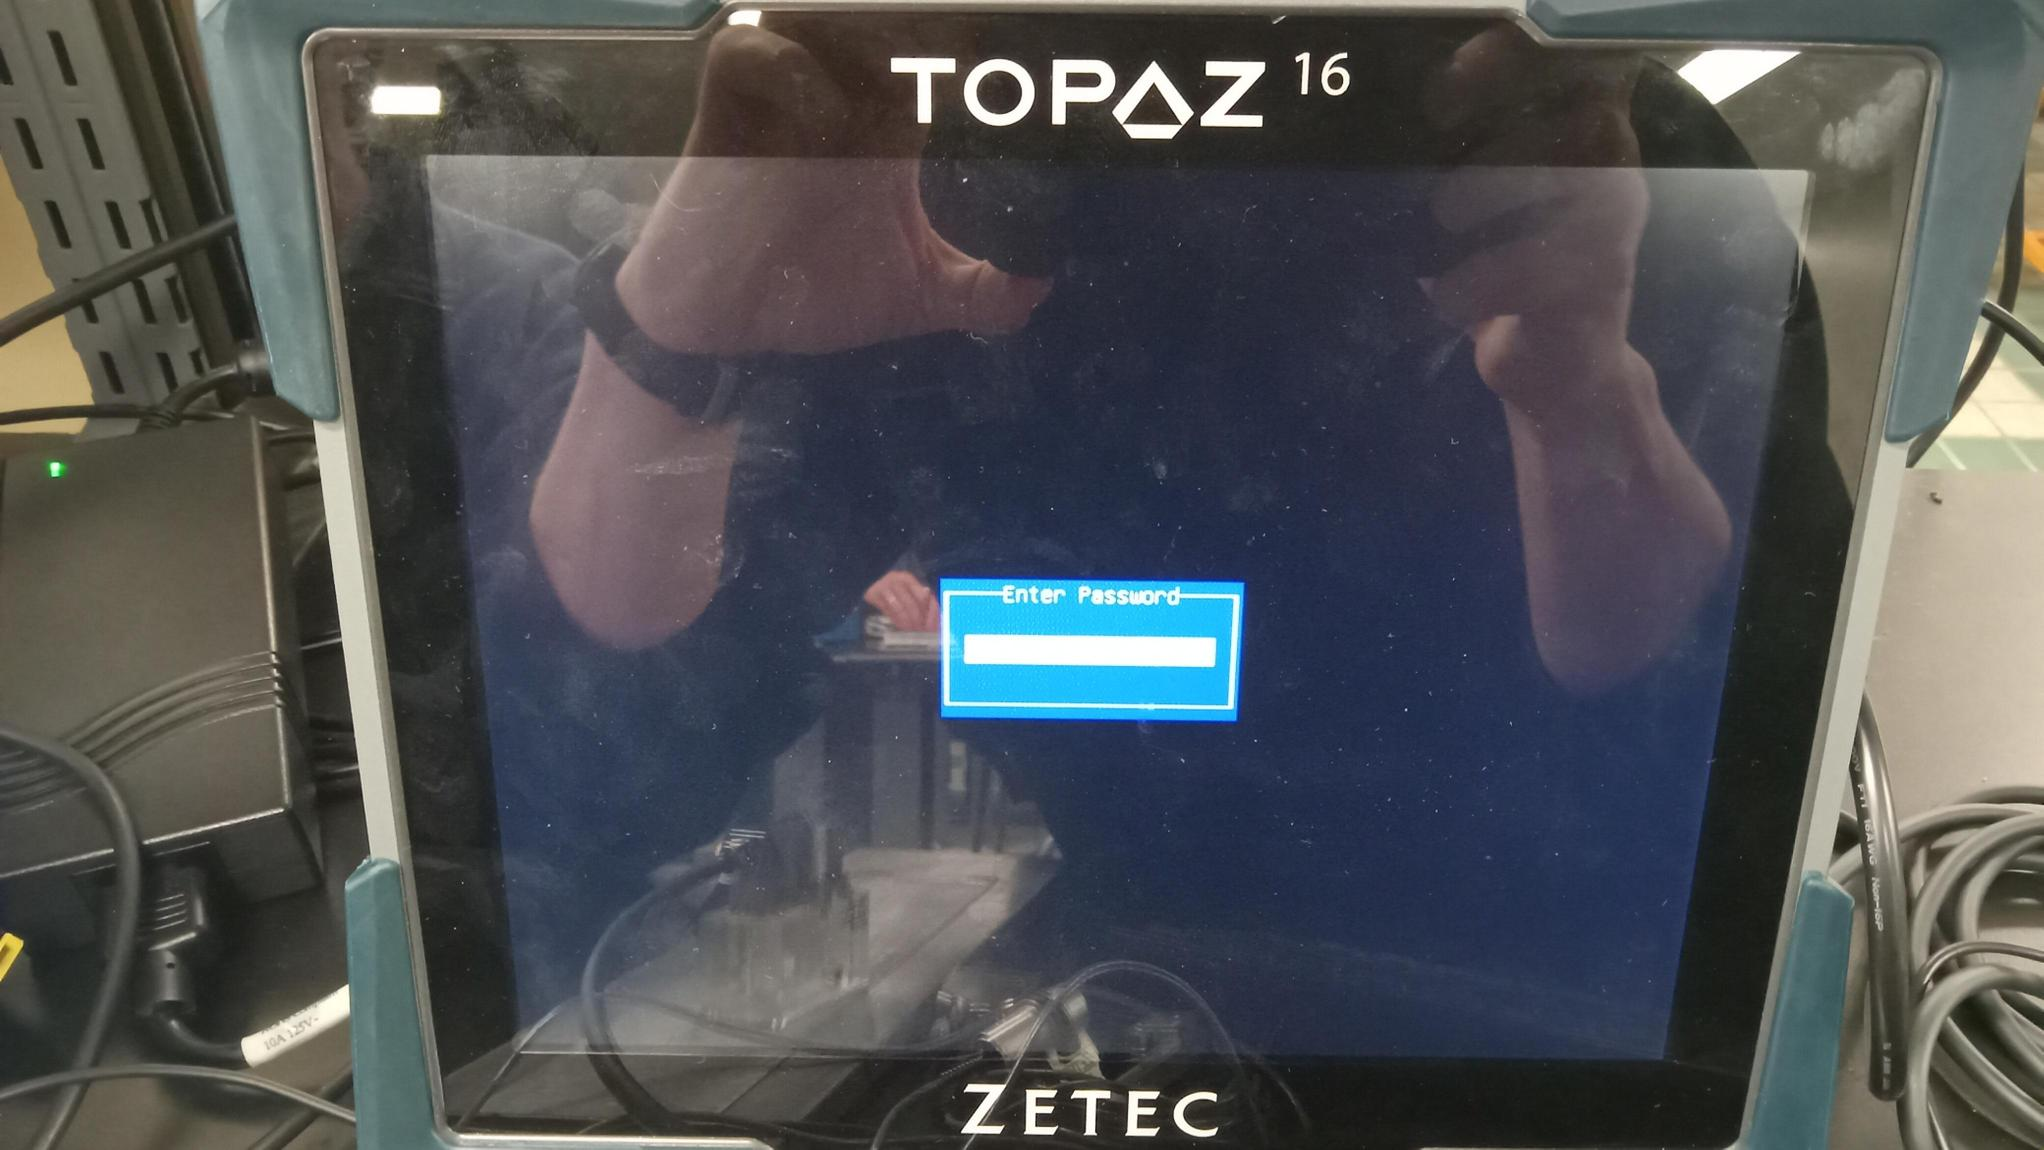
\includegraphics[width=\textwidth]{../../figures/Photos_Lab/Bios2.jpg}
  \caption{}
  \label{fig:bios-mdp}
\end{subfigure}
\hfill
\begin{subfigure}[t]{0.32\textwidth}
  \centering
  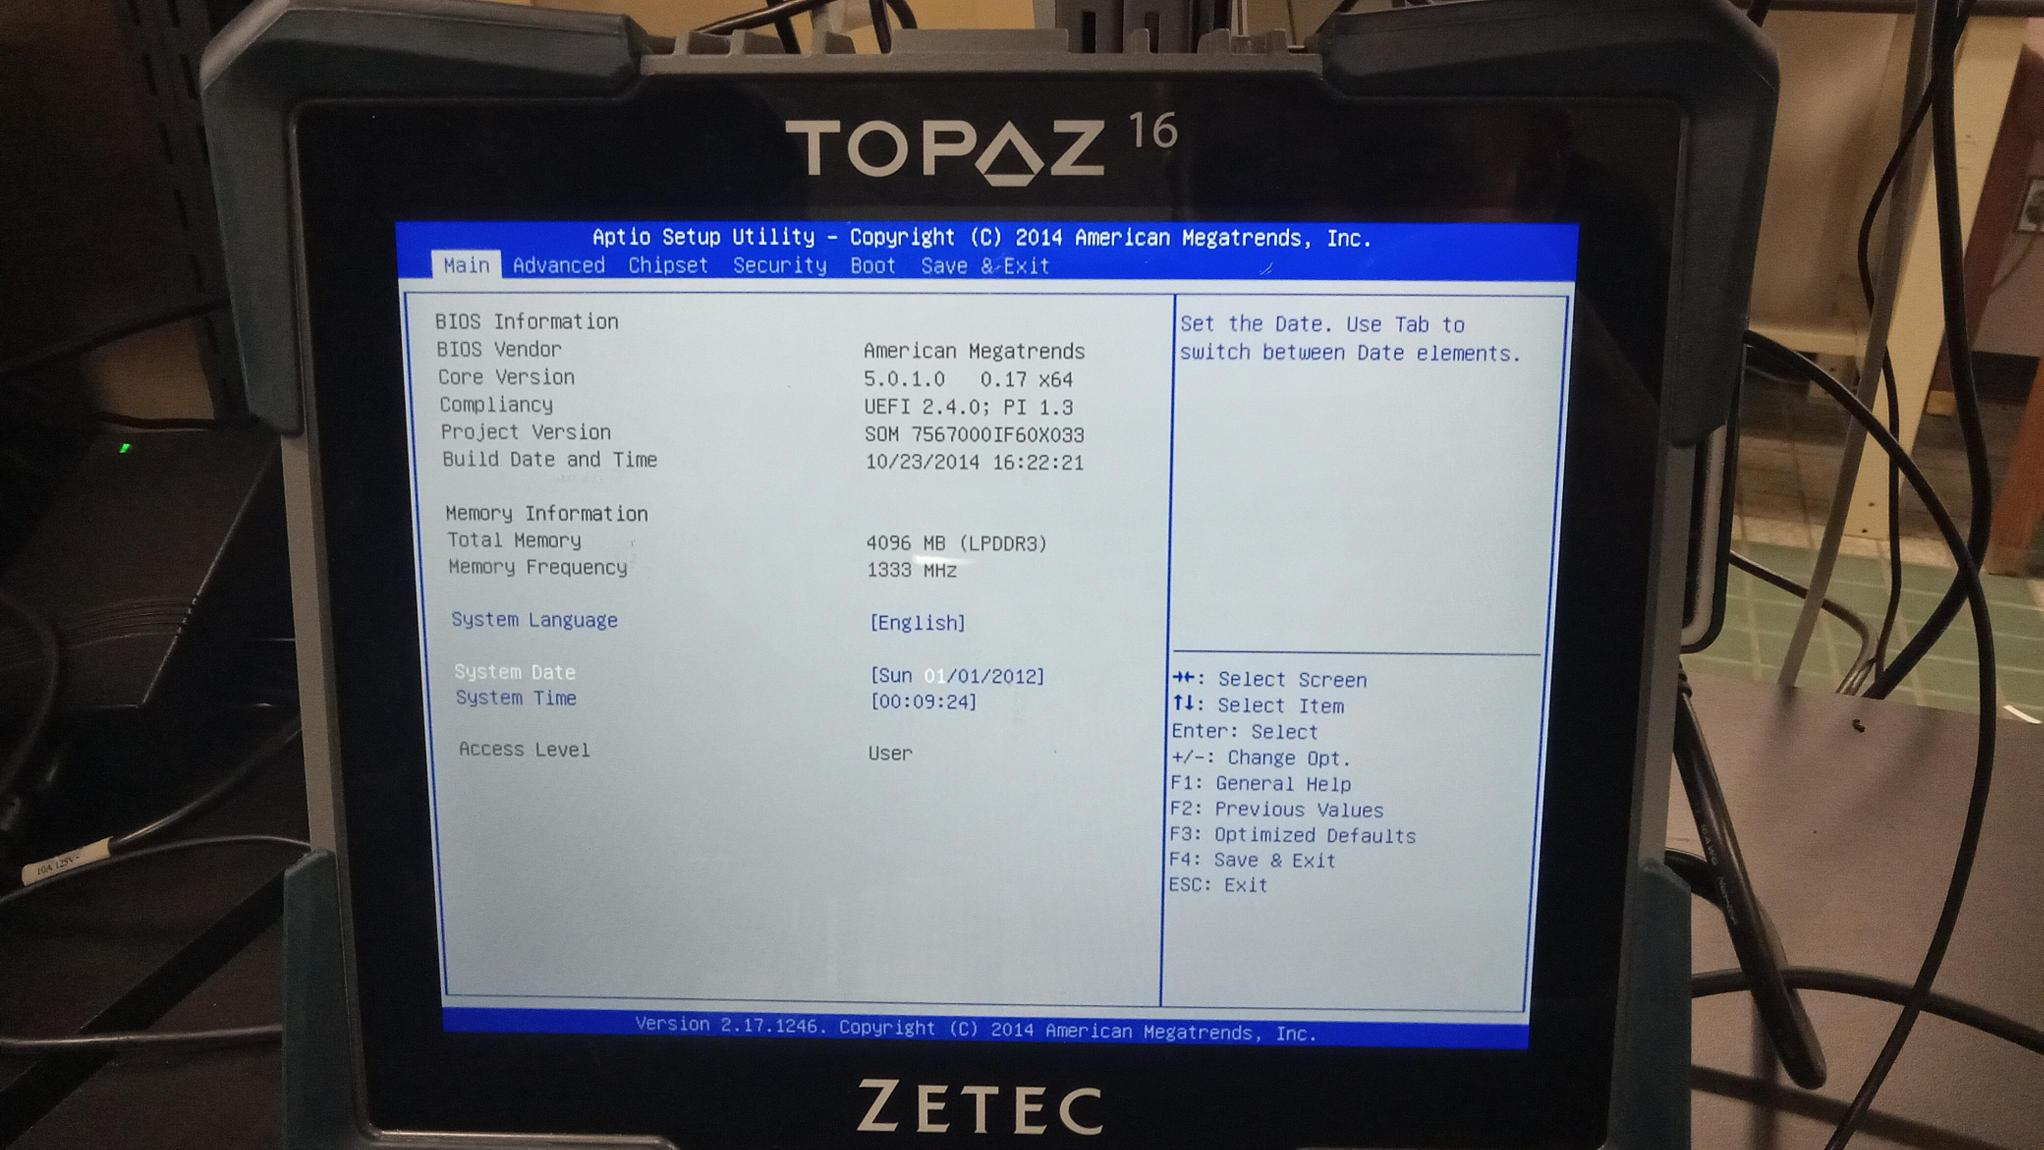
\includegraphics[width=\textwidth]{../../figures/Photos_Lab/Bios3.jpg}
  \caption{}
  \label{fig:bios-page}
\end{subfigure}
\caption{\'Ecran de d\'emarrage, appuyer sur Suppr ou \'Echap (a). Fen\^etre Enter Password, appuyer sur Enter (b). Page du BIOS, choisir Save and Exit (c).}
\label{fig:bios}
\end{figure}

\subsection{Connexion de la sonde}

Pour connecter la sonde phase array, retirer d'abord le capot de protection du connecteur en faisant glisser le loquet de la position verrouill\'ee vers la position d\'everrouill\'ee. Aligner ensuite le connecteur de la sonde avec celui du panneau lat\'eral et verrouiller le loquet.

\begin{figure}[H]
\centering
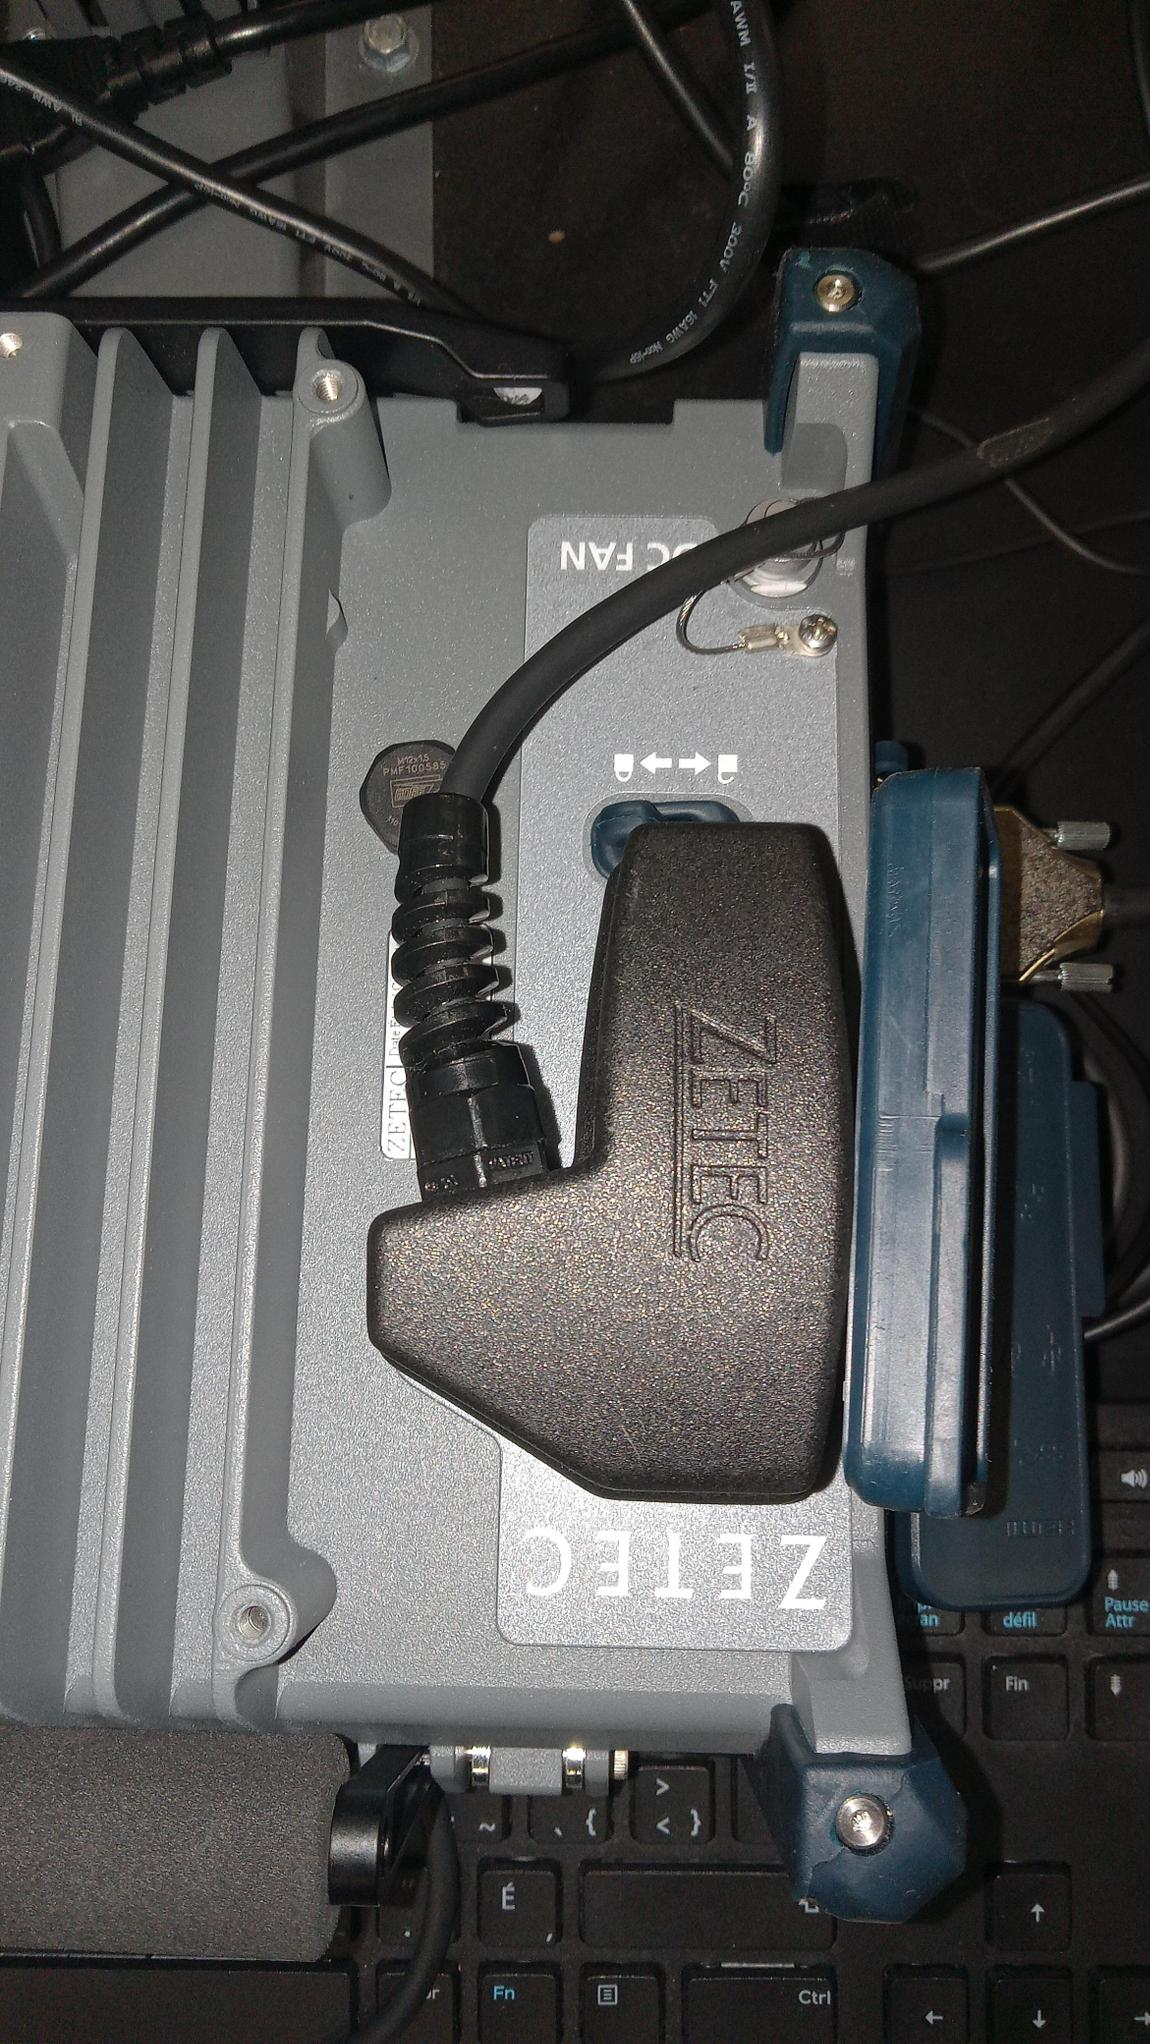
\includegraphics[height=9cm]{../../figures/Photos_Lab/ConnecteurSonde.jpg}
\caption{Connexion de la sonde phase array.}
\label{fig:connexion-sonde}
\end{figure}

Si le connecteur de la sonde est reconnu par l'appareil, le Topaz la d\'etecte au branchement et affiche la fen\^etre New Probe Detected. Le manuel recommande de choisir la configuration du canal avant de brancher la sonde, pour que cette d\'etection se fasse correctement. Si la sonde n'est pas d\'ej\`a branch\'ee en d\'ebut de s\'eance, il vaut donc mieux attendre l'\'etape~2 de la Section~\ref{sec:configuration} pour la brancher.

\begin{figure}[H]
\centering
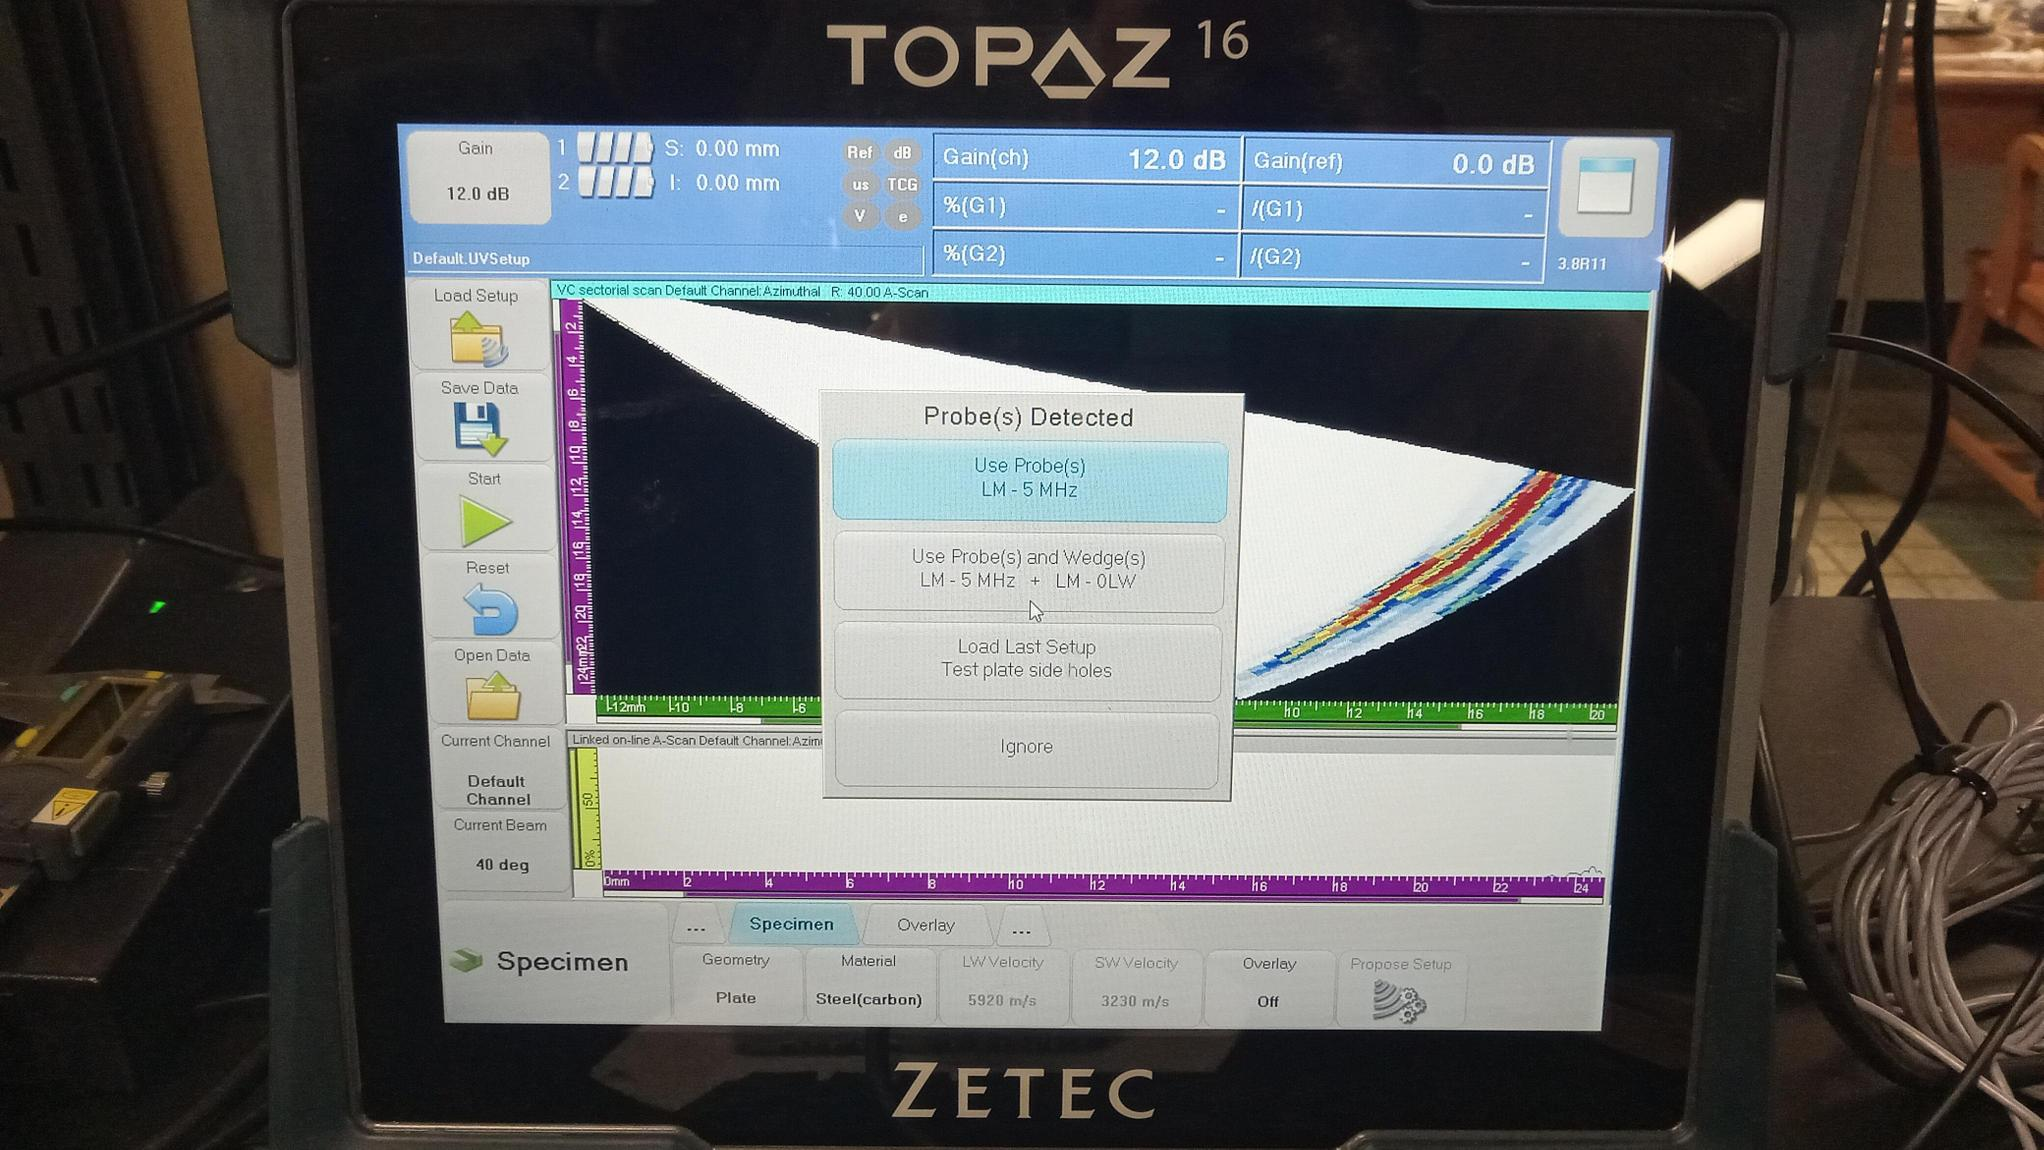
\includegraphics[width=10cm]{../../figures/Photos_Lab/EcranConnectionSonde1.jpg}
\caption{Fen\^etre Probe(s) Detected.}
\label{fig:sonde-detectee}
\end{figure}

\subsection{Interface UltraVision Touch}

Une fois la s\'equence de d\'emarrage termin\'ee, l'interface UltraVision Touch appara\^it. Elle est organis\'ee en quelques zones principales: le nom du fichier ouvert et le r\'eglage du gain en haut, une zone d'information sur l'\'etat de l'appareil (charge de la batterie, \'etat des calibrations), la zone d'affichage des donn\'ees au centre, puis en bas un menu permettant de choisir la fonction voulue (sp\'ecimen, canal, calibration, etc.) et des sous-menus donnant acc\`es aux param\`etres de cette fonction.

\begin{figure}[H]
\centering
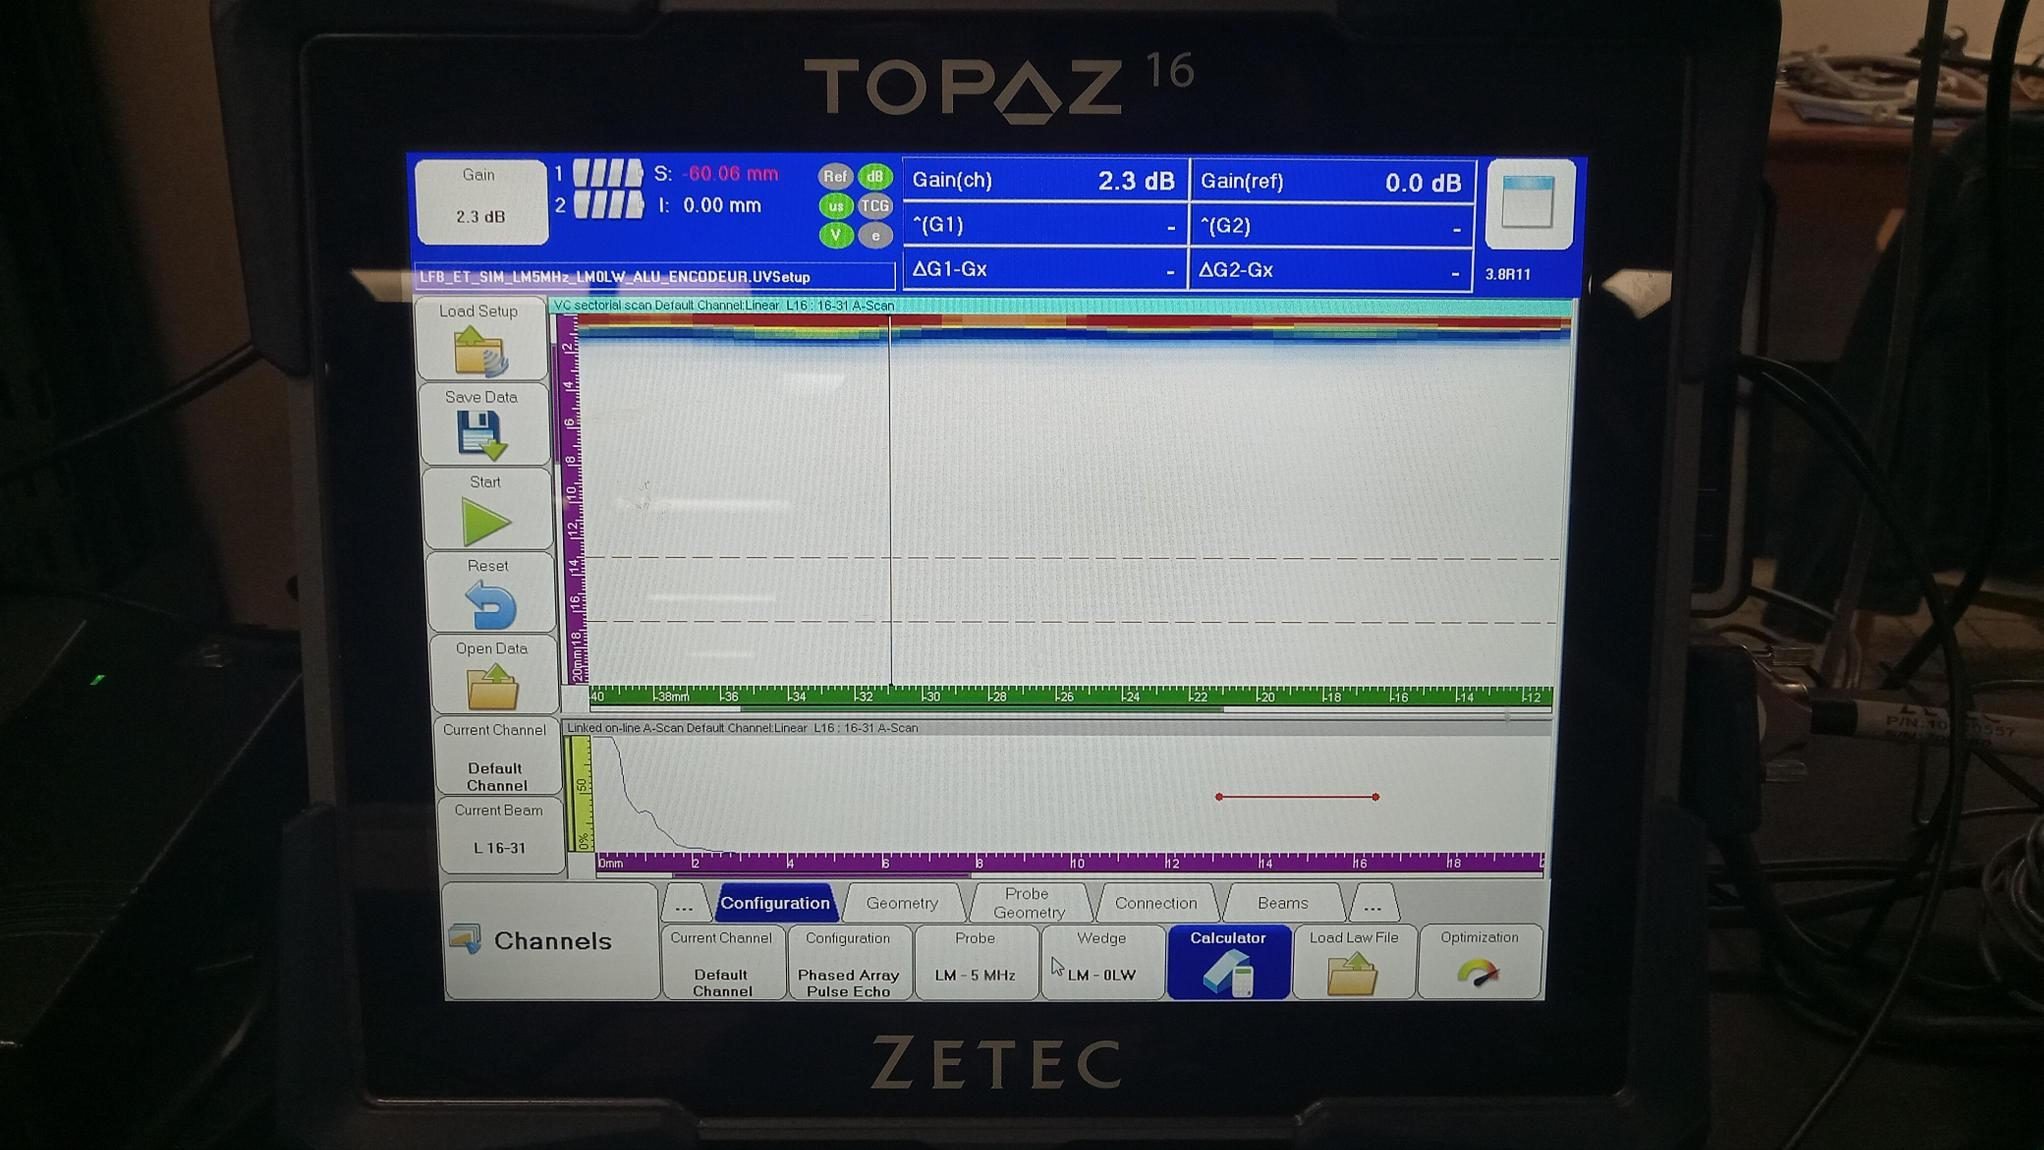
\includegraphics[width=10cm]{../../figures/Photos_Lab/Ecran1.jpg}
\caption{Fen\^etre principale d'UltraVision Touch.}
\label{fig:interface}
\end{figure}

Les indicateurs de calibration, dans la zone d'\'etat, sont gris tant qu'aucune calibration n'a \'et\'e faite, jaunes si elle est incompl\`ete pour certains faisceaux et verts lorsqu'elle est compl\`ete pour tous les faisceaux de la configuration. Ces indicateurs permettent de v\'erifier rapidement l'\'etat de calibration avant de commencer une acquisition.

\subsection{Configuration d'une inspection}
\label{sec:configuration}

Avant de pouvoir calibrer l'appareil ou faire une mesure, une configuration d'inspection doit \^etre d\'efinie dans UltraVision Touch. Les valeurs donn\'ees dans cette section sont celles de la configuration utilis\'ee au laboratoire avec la sonde lin\'eaire LM de Zetec (5~MHz, 64~\'el\'ements) et le sabot droit LM-0LW. Les noms de menus et de boutons sont ceux de l'interface en anglais, tels qu'ils apparaissent \`a l'\'ecran.

\subsubsection*{Option rapide: charger la configuration du laboratoire}

Si le fichier LFB\_ET\_SIMlT\_LM5MHz\_LM0LW\_ALU.UVSetup est pr\'esent dans le dossier Setups de l'appareil, il suffit de le charger: menu File, bouton Load Setup, choisir le fichier, puis Accept. Toutes les valeurs des tableaux qui suivent sont alors d\'ej\`a entr\'ees. Il reste \`a v\'erifier l'\'epaisseur de la pi\`ece dans le menu Specimen (\'etape~1) et \`a refaire la calibration (Section~\ref{sec:calibration}), qui doit \^etre refaite \`a chaque s\'eance. Les \'etapes suivantes permettent de refaire la configuration au complet, ou de v\'erifier celle qui a \'et\'e charg\'ee.

\begin{figure}[H]
\centering
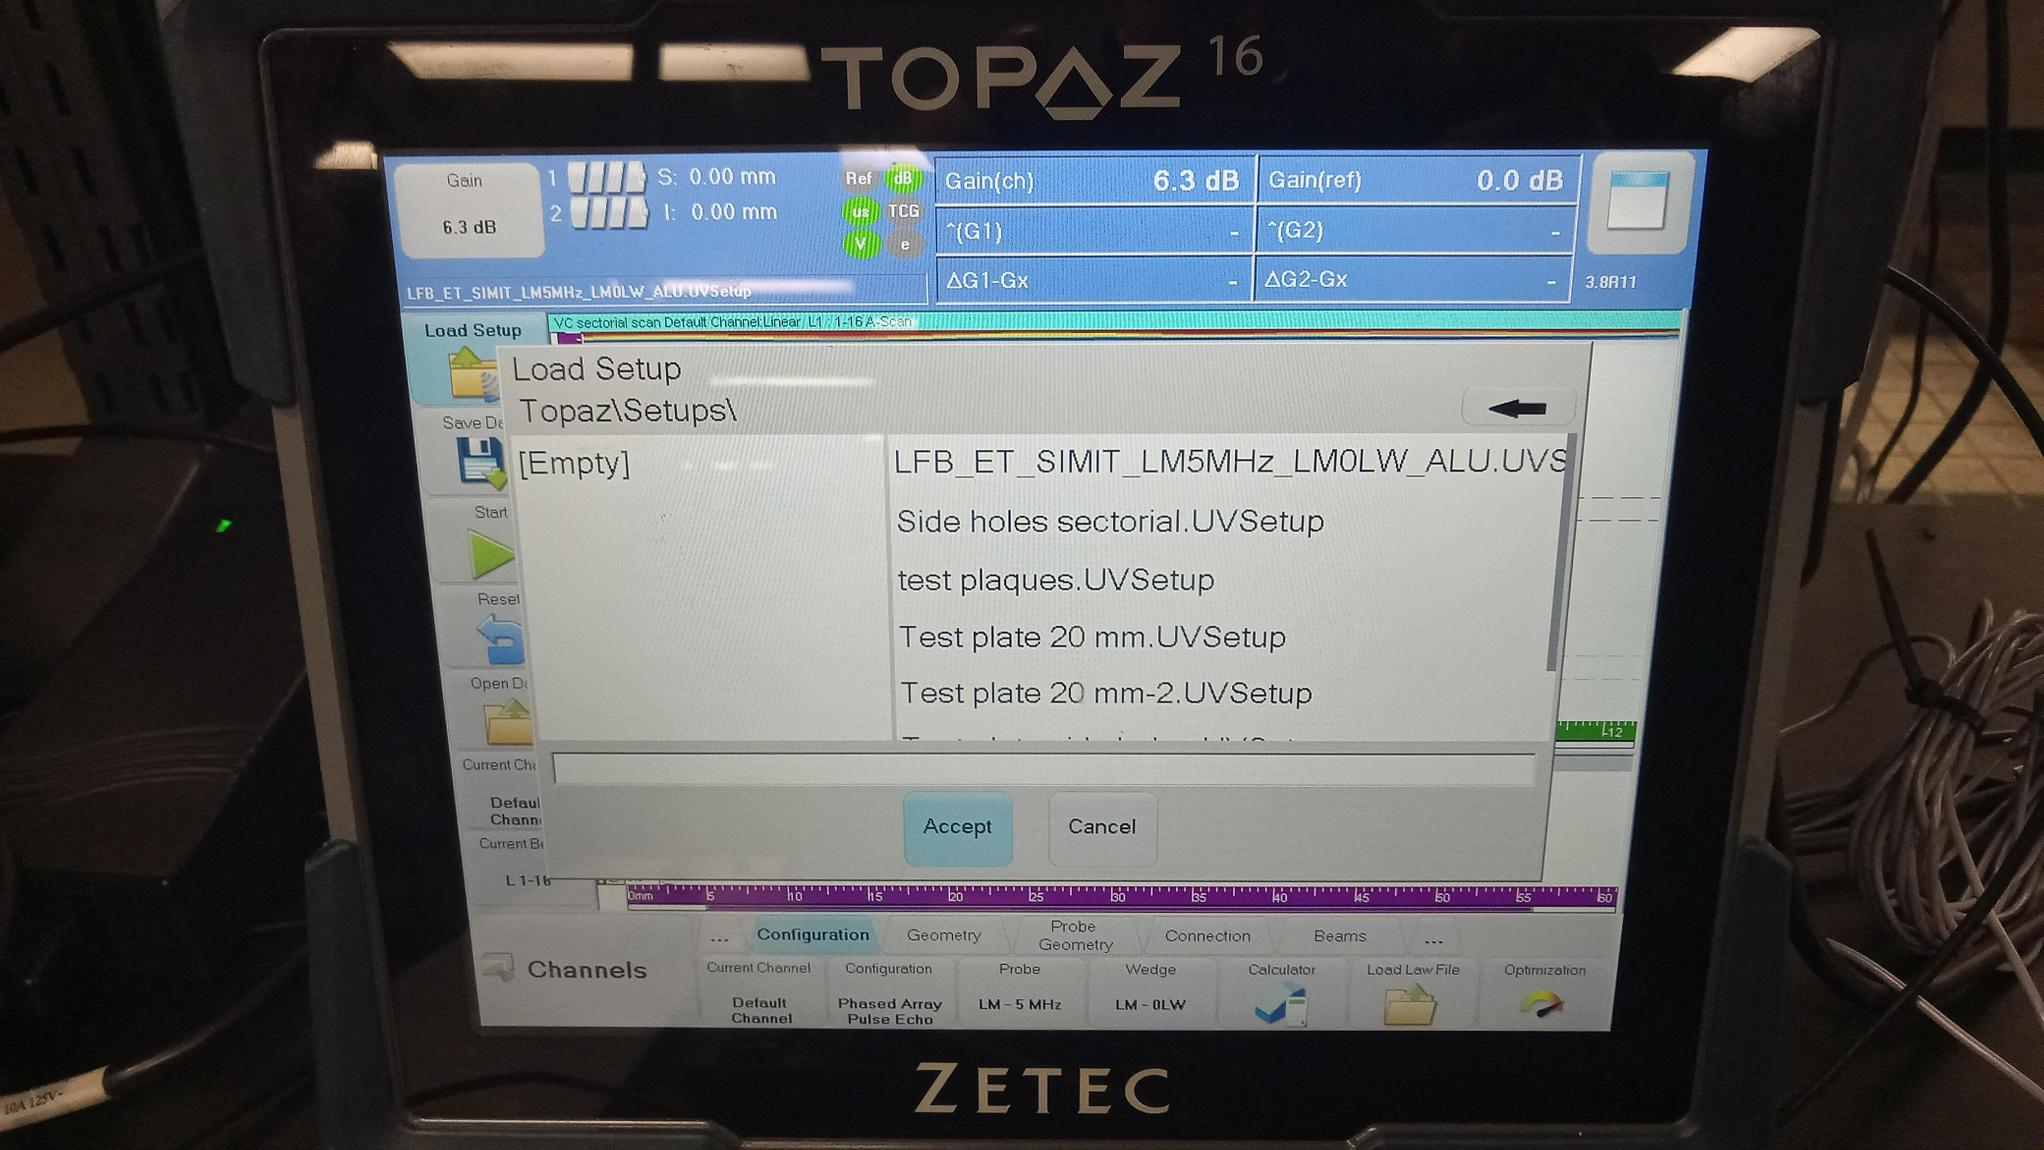
\includegraphics[width=10cm]{../../figures/Photos_Lab/SauvegardeSetup1.jpg}
\caption{Fen\^etre Load Setup avec la liste des configurations.}
\label{fig:load-setup}
\end{figure}

\subsubsection*{\'Etape 1: d\'efinir le sp\'ecimen}

\begin{enumerate}
  \item Appuyer sur le bouton de s\'election du menu (en bas de l'\'ecran) et choisir Specimen.
  \item Appuyer sur Geometry. Dans la fen\^etre Shape Editor, r\'egler les param\`etres du Tableau~\ref{tab:specimen}, puis appuyer sur Accept.
  \item Appuyer sur Material, choisir l'aluminium dans la liste, puis Accept. Les champs LW Velocity et SW Velocity doivent afficher les vitesses du Tableau~\ref{tab:specimen}.
\end{enumerate}

\begin{table}[H]
\centering
\caption{Param\`etres du sp\'ecimen (menu Specimen).}
\label{tab:specimen}
\begin{tabular}{ll}
\toprule
Param\`etre & Valeur \\
\midrule
Shape Type & Plate \\
Weld Type & None \\
Thickness & \'epaisseur mesur\'ee \\
Material & aluminium \\
LW Velocity & 6320~m/s \\
SW Velocity & 3130~m/s \\
\bottomrule
\end{tabular}
\end{table}

\subsubsection*{\'Etape 2: d\'efinir le canal, la sonde et le sabot}

\begin{enumerate}
  \item Choisir le menu Channel. Appuyer sur Configuration et choisir Phased Array-Pulse Echo. Le manuel recommande de faire ce choix avant de brancher la sonde.
  \item Si la sonde n'est pas encore branch\'ee, la brancher comme d\'ecrit \`a la section pr\'ec\'edente. Si la fen\^etre New Probe Detected appara\^it, appuyer sur Use Probe and Wedge, puis choisir le sabot LM-0LW dans la liste.
  \item Si la sonde \'etait d\'ej\`a branch\'ee, ou si la fen\^etre New Probe Detected n'appara\^it pas, appuyer sur Probe, puis Database, et choisir la sonde LM de 5~MHz \`a 64~\'el\'ements. Appuyer ensuite sur Wedge, puis Database, et choisir LM-0LW.
  \item Si la sonde ou le sabot n'apparaissent pas dans la base de donn\'ees, les d\'efinir \`a la main avec Probe, puis Edit (ou Wedge, puis Edit), en entrant les valeurs du Tableau~\ref{tab:sonde}.
\end{enumerate}

\begin{table}[H]
\centering
\caption{Caract\'eristiques de la sonde et du sabot du laboratoire.}
\label{tab:sonde}
\begin{tabular}{lll}
\toprule
& Param\`etre & Valeur \\
\midrule
Sonde & Type & Linear \\
& Frequency & 5~MHz \\
& Element Quantity & 64 \\
& Pitch & 0,6~mm \\
& Primary Axis Element Size & 0,5~mm \\
& Secondary Axis Element Size & 10~mm \\
\midrule
Sabot & Name & LM-0LW \\
& Wave Type & Longitudinal \\
& Wedge Angle & 0\textdegree \\
& Length $\times$ Width $\times$ Height & $51 \times 28 \times 30$~mm \\
& First Element Height & 30~mm \\
& First Element Primary Axis Offset & 6,6~mm \\
& First Element Secondary Axis Offset & 14~mm \\
& Velocity & 2330~m/s \\
\bottomrule
\end{tabular}
\end{table}

\subsubsection*{\'Etape 3: d\'efinir la loi focale}

Dans le menu Channel, appuyer sur Calculator, r\'egler les param\`etres du Tableau~\ref{tab:calculateur}, puis appuyer sur Accept. Chaque fois qu'un param\`etre de la sonde, du sabot ou de la loi focale change, le message \og Focal law parameters have been changed \fg{} appara\^it: appuyer alors sur Recompute.

\begin{table}[H]
\centering
\caption{Param\`etres de la loi focale (fen\^etre Calculator).}
\label{tab:calculateur}
\begin{tabular}{llp{7.5cm}}
\toprule
Param\`etre & Valeur & Remarque \\
\midrule
Skew Angle & 90\textdegree & valeur utilis\'ee au laboratoire \\
Scan Reference & d\'efaut & \\
Index Reference & d\'efaut & \\
Wave Type & Longitudinal & compatible avec le sabot droit \\
Sweep & Linear & l'ouverture se d\'eplace le long du r\'eseau \\
Angle & 0\textdegree & incidence normale \\
Aperture & 16 & nombre maximal d'\'el\'ements actifs du Topaz du laboratoire \\
First Element & 1 & \\
Last Element & 64 & \\
Focal Point & Half Path & \\
Position & 20~mm & profondeur de focalisation \\
Timebase Type & True Depth & axe vertical gradu\'e en profondeur \\
Timebase Start & 0~mm & \\
Timebase Range & 60~mm & au moins $2e + 5$~mm, pour voir le deuxi\`eme \'echo de fond d'un bloc d'\'epaisseur $e$. 60~mm convient \`a un bloc d'environ 25~mm, et une plage plus longue donne des fichiers de donn\'ees plus lourds \\
\bottomrule
\end{tabular}
\end{table}

Avec ces valeurs, l'ouverture de 16~\'el\'ements se d\'eplace d'un \'el\'ement \`a la fois de la position 1 \`a 16 jusqu'\`a la position 49 \`a 64, ce qui donne $64 - 16 + 1 = 49$ faisceaux. UltraVision Touch les nomme L~1-16 \`a L~49-64.

\begin{figure}[H]
\centering
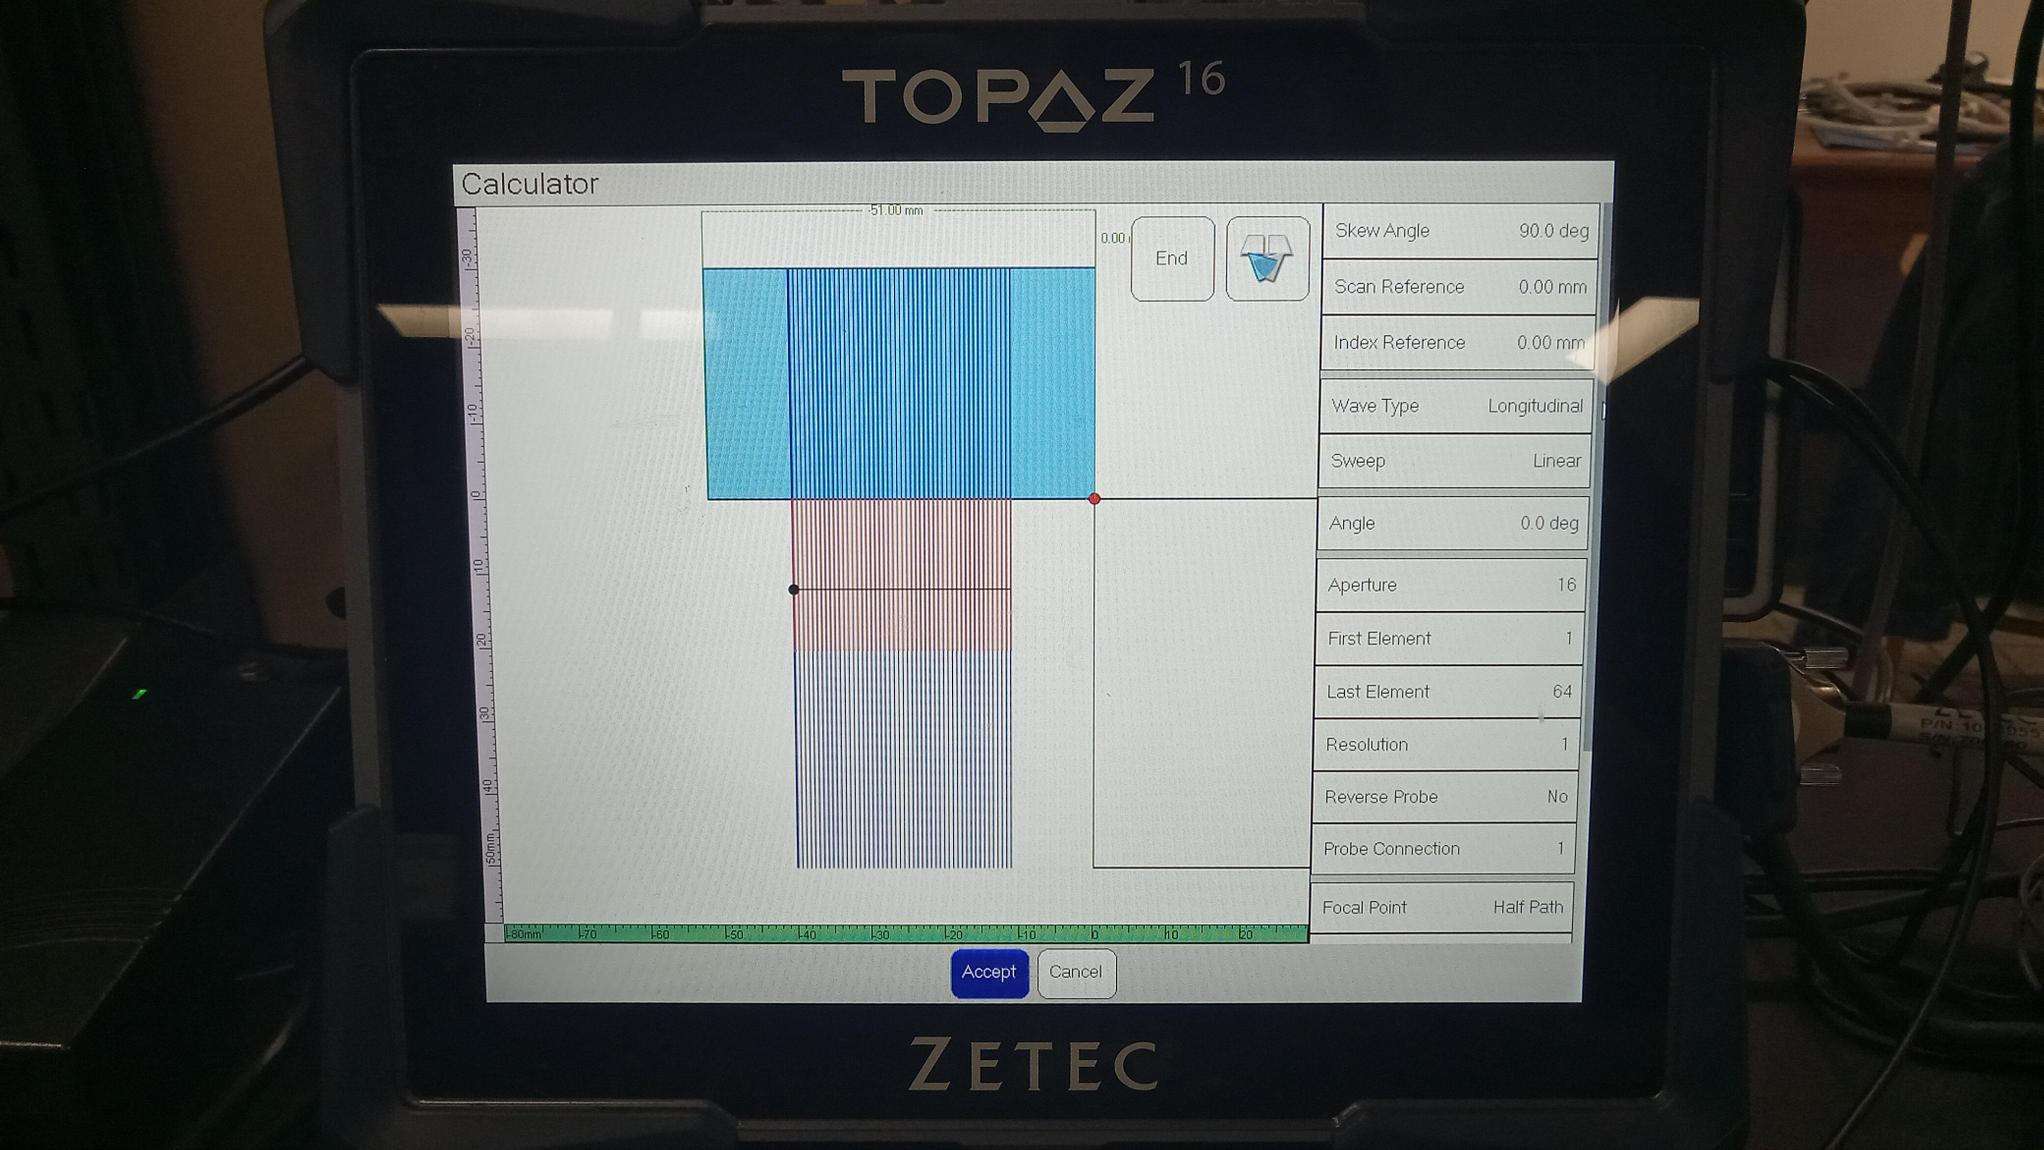
\includegraphics[width=10cm]{../../figures/Photos_Lab/Calculateur.jpg}
\caption{Fen\^etre Calculator dans UltraVision Touch.}
\label{fig:calculateur}
\end{figure}

\subsubsection*{\'Etape 4: r\'eglages ultrasonores}

Dans le menu UT Settings, r\'egler les param\`etres du Tableau~\ref{tab:ut}. Le gain est ensuite ajust\'e avec le bouton Gain en haut de l'\'ecran, en posant la sonde avec du couplant sur le bloc: l'\'echo de fond doit atteindre environ 80~\% de la hauteur de l'\'ecran sans saturer.

\begin{table}[H]
\centering
\caption{R\'eglages ultrasonores (menu UT Settings).}
\label{tab:ut}
\begin{tabular}{lllp{5cm}}
\toprule
Sous-menu & Param\`etre & Valeur & Remarque \\
\midrule
General & Gain & environ 6~dB & d\'epend de l'appareil et du bloc, r\'egler sur l'\'echo de fond \`a 80~\% \\
Pulser \& Receiver & Pulse Width & 100~ns & demi-p\'eriode \`a 5~MHz (ou Auto) \\
& Filter & 2 \`a 10~MHz & passe-bande \\
& Rectification & Bipolar & valeur absolue du signal (redress\'e) \\
Digitizer & Recurrence & 2500~Hz & fr\'equence de r\'ep\'etition des tirs \\
\bottomrule
\end{tabular}
\end{table}

Le mode de rectification RF affiche le signal sans rectification. Il sert \`a voir la forme d'onde et la phase de l'\'echo. Ce mode n'a pas \'et\'e test\'e dans le cadre de ce guide.

\subsubsection*{\'Etape 5: s\'equence d'acquisition}

Sans encodeur, la sonde est d\'eplac\'ee \`a la main et sa position n'est pas mesur\'ee. Dans le menu Mechanical, r\'egler Sequence Type \`a One Line, puis, dans le sous-menu Encoder, r\'egler Encoder ID \`a Clock: la position de balayage avance alors avec l'horloge interne de l'appareil. Si l'affichage d\'efile trop vite, diminuer Acquisition Rate dans UT Settings, sous-menu Digitizer.

Scan Start, Scan Stop et la r\'esolution de scan d\'efinissent un tampon de positions. Par exemple, de 0 \`a 100~mm avec une r\'esolution de 0,25~mm, on obtient 401 positions. \`A une fr\'equence d'acquisition de 20~Hz, ce tampon est rempli en 20~s.

Le tampon est circulaire. Si l'acquisition dure plus longtemps que ce qu'il peut contenir, le Topaz r\'e\'ecrit le d\'ebut du fichier avec les derni\`eres positions. Il faut donc un Scan Stop assez grand pour tout le passage (par exemple 150~mm, soit 30~s \`a 20~Hz), et appuyer sur Stop (le gros bouton rouge \`a c\^ot\'e de Start) d\`es la fin du d\'eplacement.

Fixer Acquisition Rate \`a une valeur pr\'ecise, par exemple 20~Hz, plut\^ot qu'\`a Max. La vitesse de d\'eplacement \`a viser est alors la r\'esolution multipli\'ee par la fr\'equence, soit $0{,}25~\text{mm} \times 20~\text{Hz} = 5$~mm/s. En pratique, des rep\`eres au ruban adh\'esif plac\'es tous les 10~mm, \`a franchir toutes les 2~s, aident \`a garder une vitesse constante.

Pour pouvoir analyser les donn\'ees plus tard (vues de coupe, 3D), il faut enregistrer les A-scans complets et pas seulement le C-scan. Dans UT Settings, sous-menu Digitizer, Record Condition doit \^etre \`a No condition, qui enregistre les A-scans complets (ne pas choisir C-Scan).

\subsubsection*{Variante avec encodeur}

Si un encodeur de position est utilis\'e, la position de balayage ne vient plus de l'horloge interne et les longueurs le long du balayage sont mesur\'ees au lieu d'\^etre estim\'ees. L'encodeur est fix\'e au sabot de la sonde (Figure~\ref{fig:sonde-encodeur}). Il ne faut pas oublier de le brancher au Topaz avant de commencer. Les r\'eglages qui changent par rapport au balayage \`a la main sont les suivants.

\begin{figure}[H]
\centering
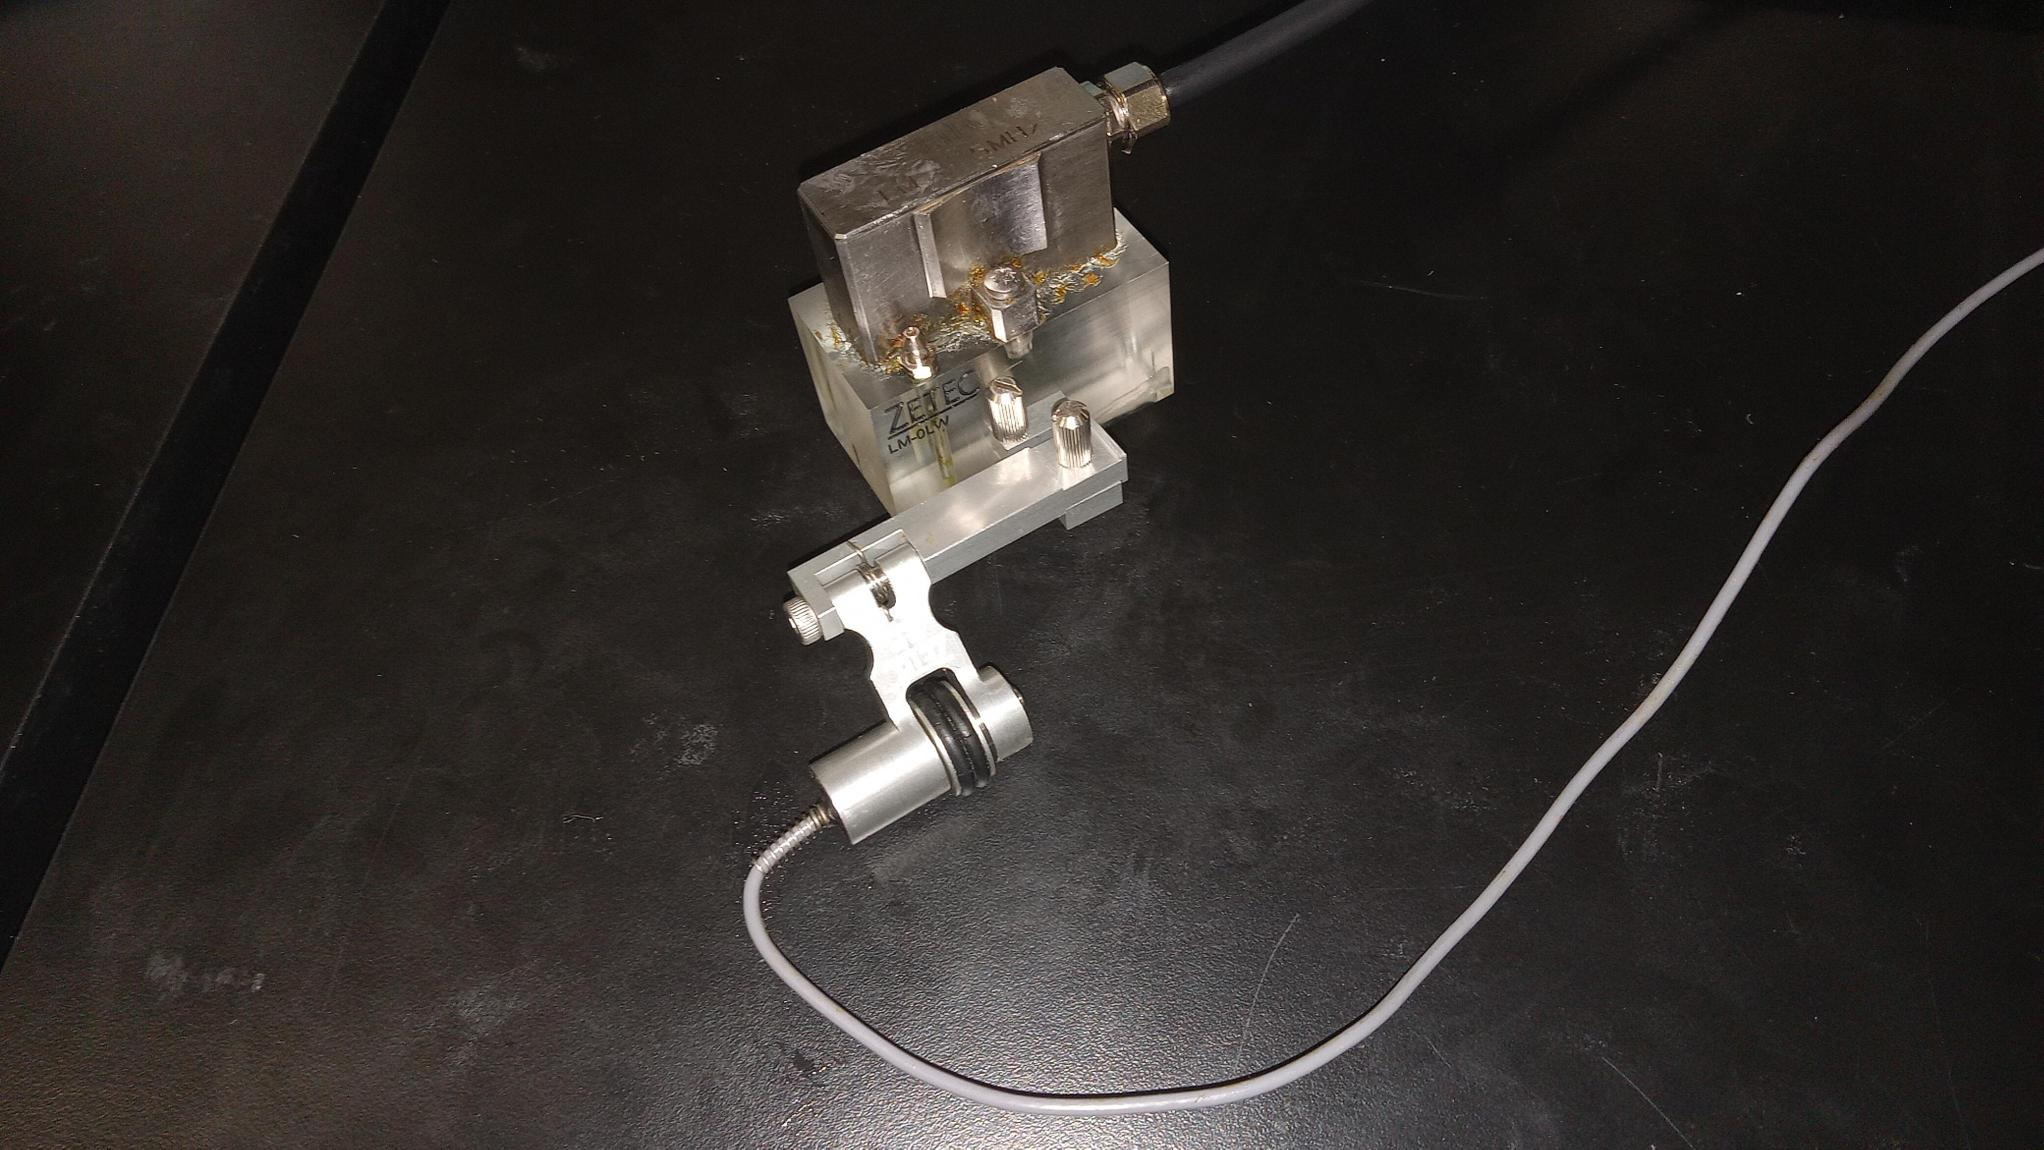
\includegraphics[width=9cm]{../../figures/Photos_Lab/SondeEncodeur1.jpg}
\caption{Sonde phase array avec son encodeur.}
\label{fig:sonde-encodeur}
\end{figure}

\begin{enumerate}
  \item Brancher l'encodeur. Le Topaz affiche la fen\^etre New Scanner Detected (Figure~\ref{fig:scanner-detecte}), avec le nom Scanner Mini-Wheel et la s\'equence One Line Scan. Appuyer sur Accept.
  \item Dans le menu Mechanical, sous-menu Scan Encoder, v\'erifier que Encoder ID est \`a~1, Type \`a Quadrature et Invert \`a Normal. La r\'esolution affich\'ee par d\'efaut est de 20~pas/mm.
  \item Calibrer l'encodeur avec le bouton Calibrate (Figure~\ref{fig:calibration-encodeur}). Dans la fen\^etre Calibrate Encoder, appuyer sur Reset, puis sur Set Start, d\'eplacer l'encodeur sur une distance mesur\'ee \`a la r\`egle (Figure~\ref{fig:methode-calibration-encodeur}), appuyer sur Set Stop, entrer cette distance avec Set Distance, puis v\'erifier Computed Resolution et appuyer sur Accept.
  \item Garder Scan Stop assez grand pour tout le passage.
  \item Dans UT Settings, sous-menu Digitizer, r\'egler Record Condition \`a No condition, qui enregistre les A-scans complets, comme pour le balayage \`a l'horloge.
  \item Dans UT Settings, sous-menu Digitizer, r\'egler Acquisition Rate \`a Max. Avec une fr\'equence fixe plus basse, il faudrait bouger tr\`es lentement: tout mouvement un peu trop rapide pendant le balayage fait sauter des positions, ce qui laisse des trous dans la mesure.
  \item Dans le menu Inspection, la valeur Max Scanning Speed est importante \`a consid\'erer: la sonde doit rester bien en dessous de cette vitesse pendant tout le balayage.
  \item Dans le menu Inspection, r\'egler Action On Start \`a Reset Encoder, pour que la position reparte de 0 \`a chaque Start.
  \item Dans UT Settings, sous-menu General, r\'eduire le Time Base Range \`a $e + 5$~mm, au lieu de $2e + 5$~mm, pour ne voir que le premier \'echo de fond et garder des fichiers plus l\'egers. Cette r\'eduction se fait seulement apr\`es la calibration (Section~\ref{sec:calibration}), qui demande de voir l'\'echo \`a $2e$. Apr\`es cette r\'eduction, les indicateurs de calibration restent verts.
\end{enumerate}

\begin{figure}[H]
\centering
\begin{subfigure}[t]{0.48\textwidth}
  \centering
  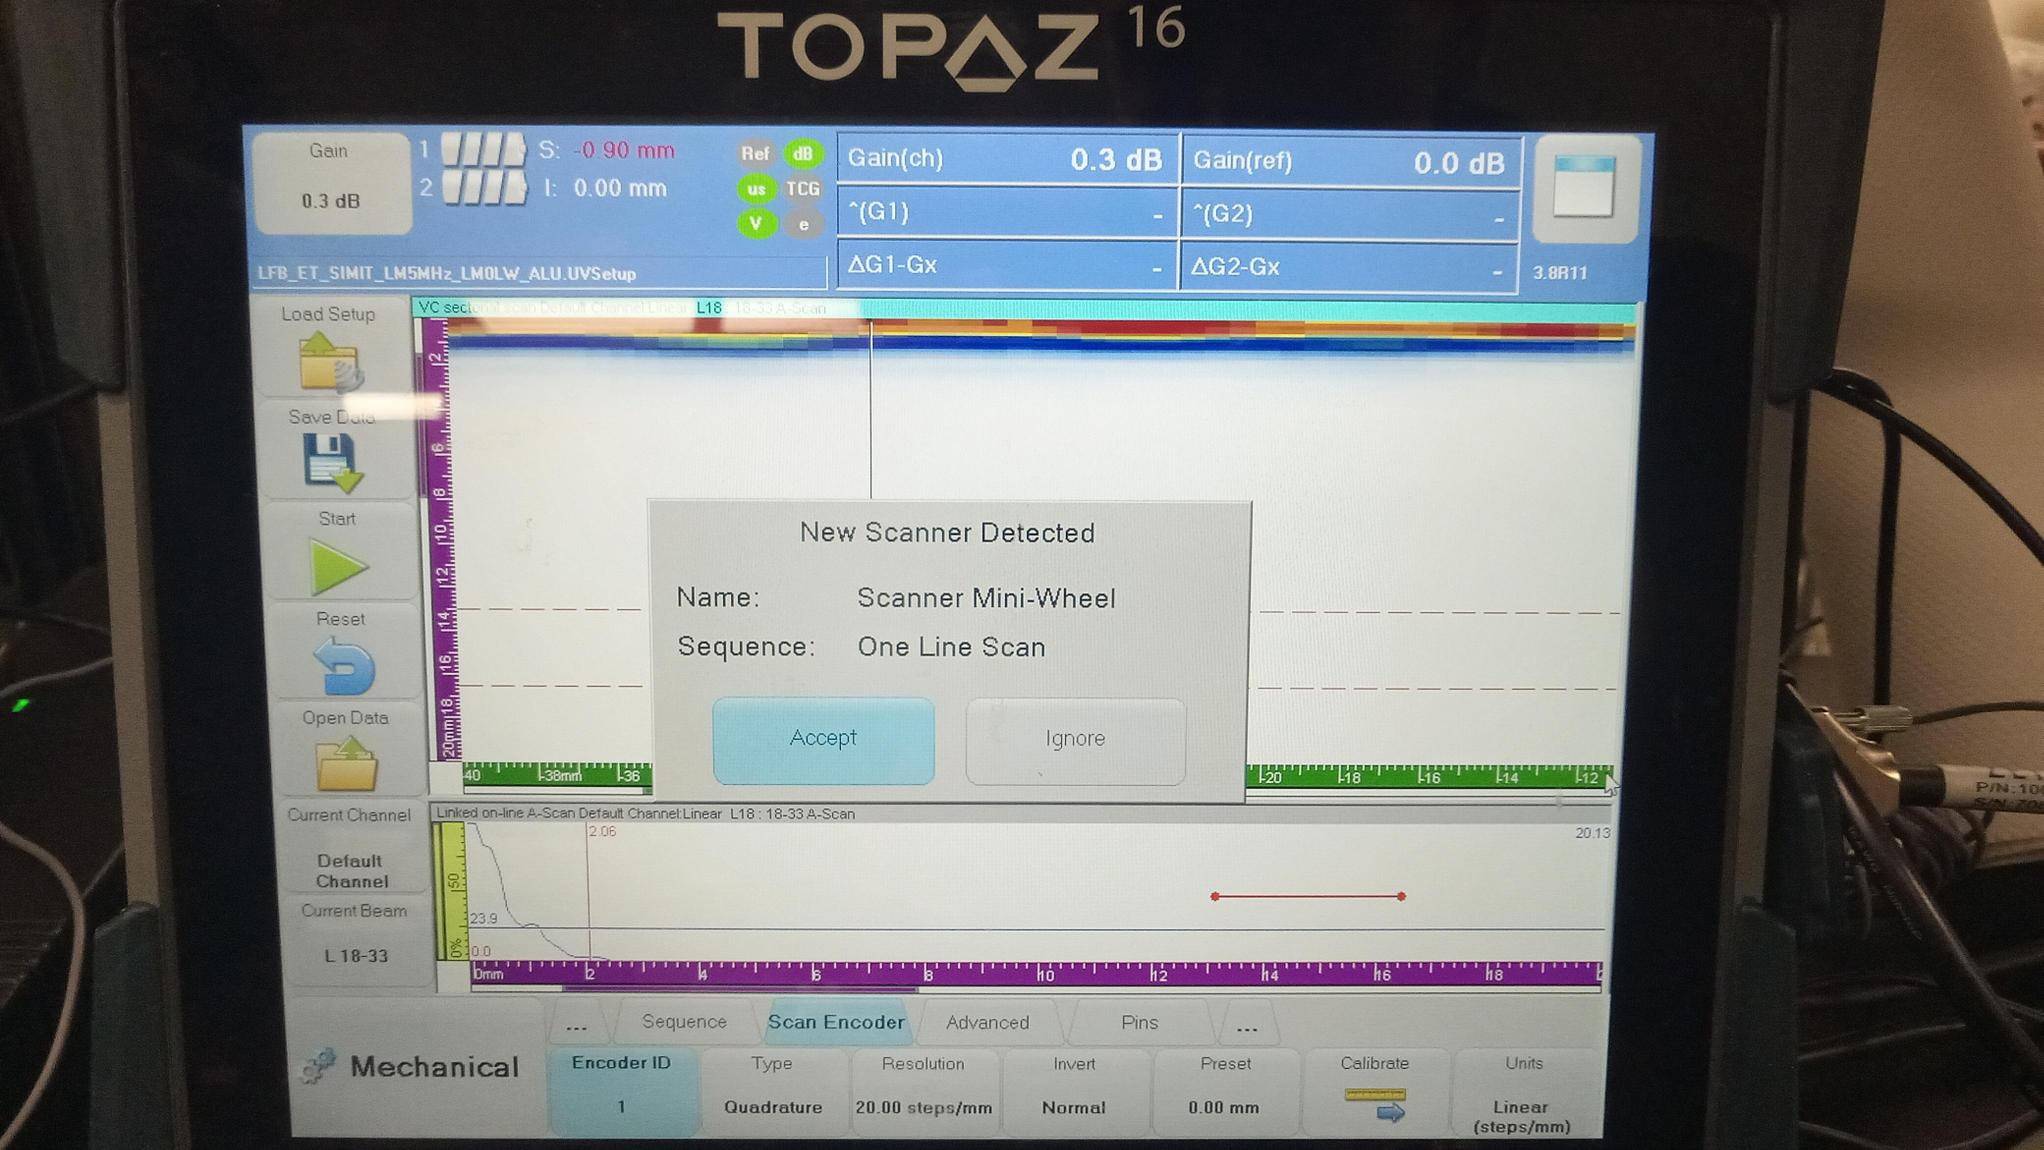
\includegraphics[width=\textwidth]{../../figures/Photos_Lab/EcranConnectionEncodeur1.jpg}
  \caption{}
  \label{fig:scanner-detecte}
\end{subfigure}
\hfill
\begin{subfigure}[t]{0.48\textwidth}
  \centering
  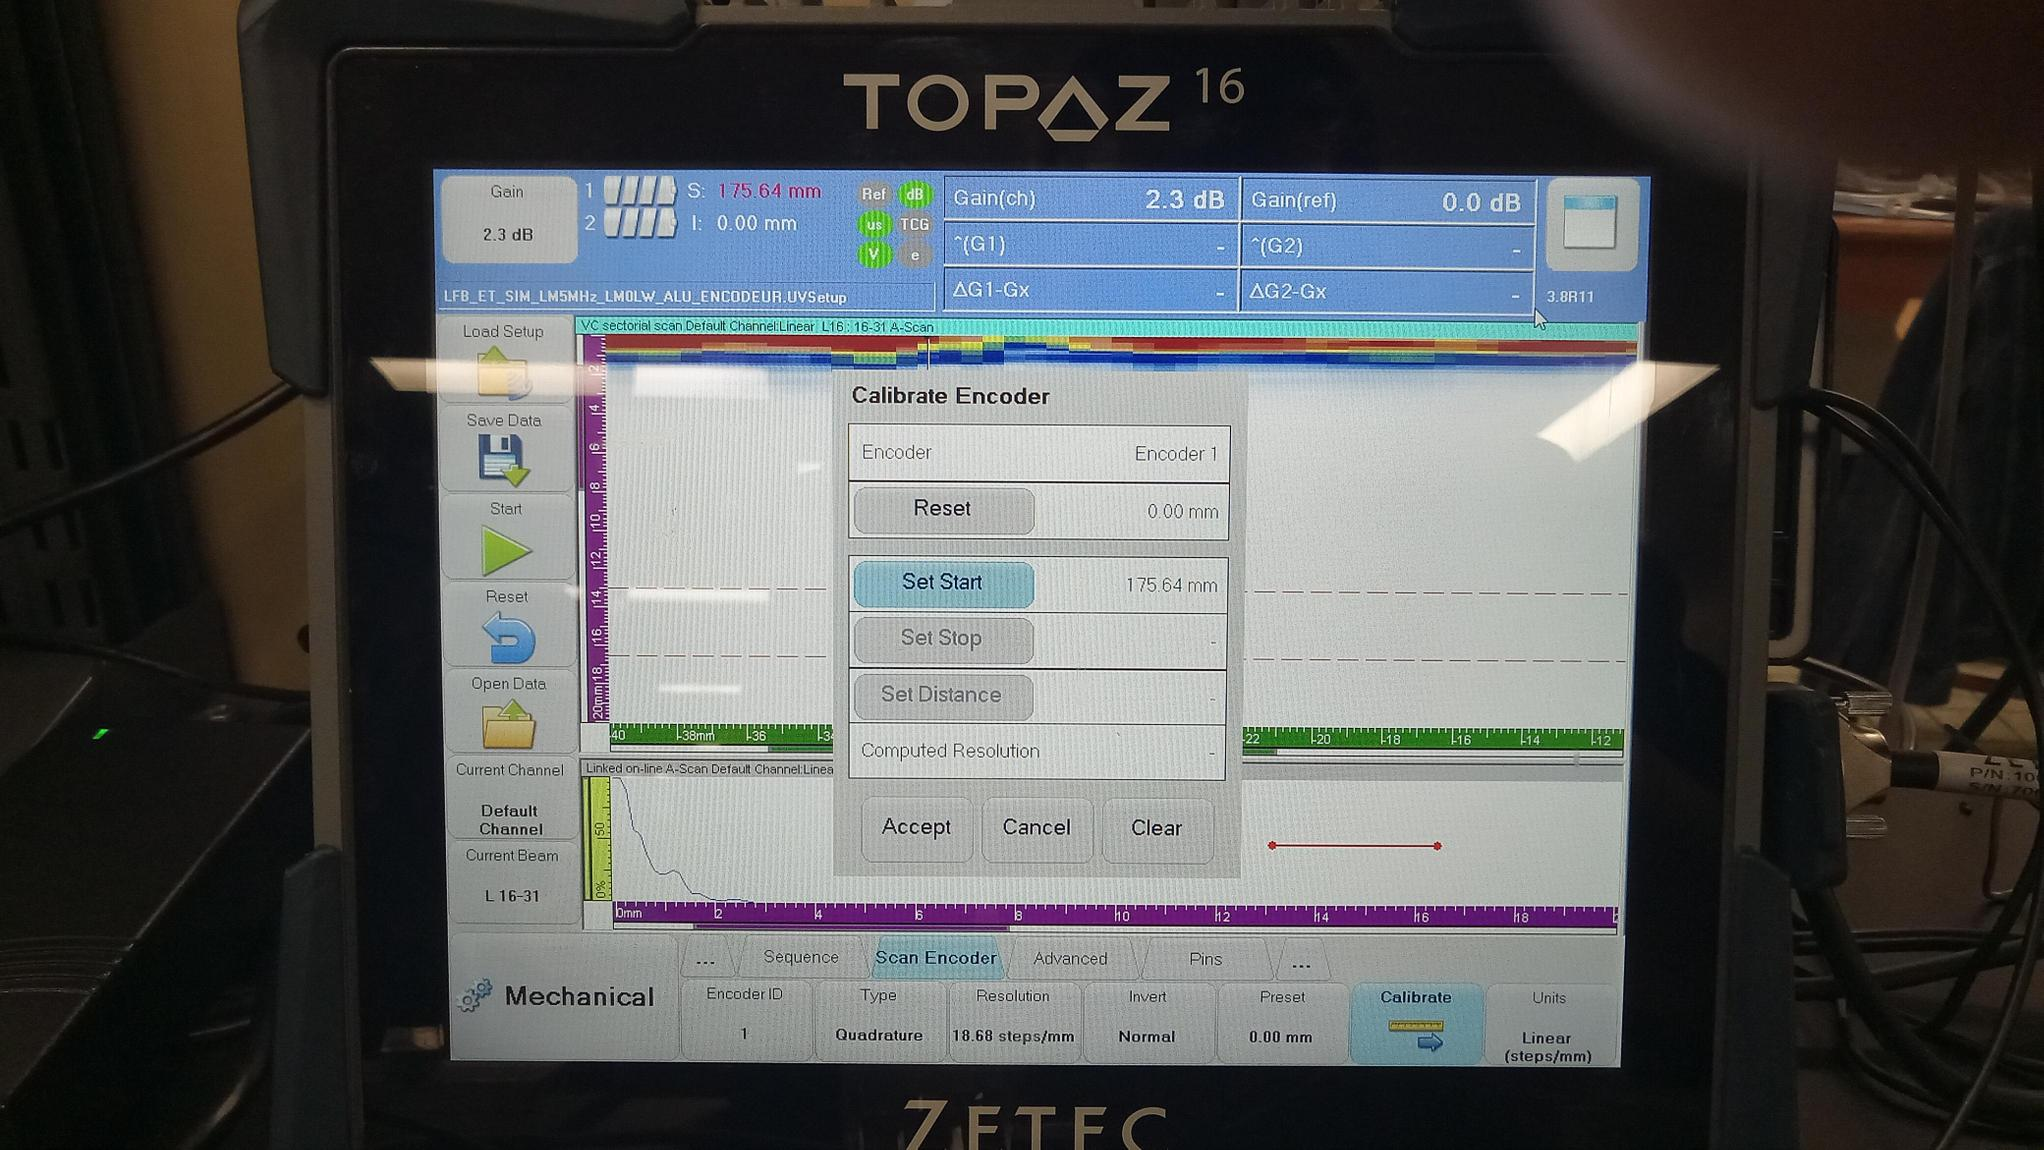
\includegraphics[width=\textwidth]{../../figures/Photos_Lab/CalibrationEncodeur1.jpg}
  \caption{}
  \label{fig:calibration-encodeur}
\end{subfigure}
\caption{D\'etection de l'encodeur (a) et fen\^etre de calibration de l'encodeur (b).}
\label{fig:ecrans-encodeur}
\end{figure}

\begin{figure}[H]
\centering
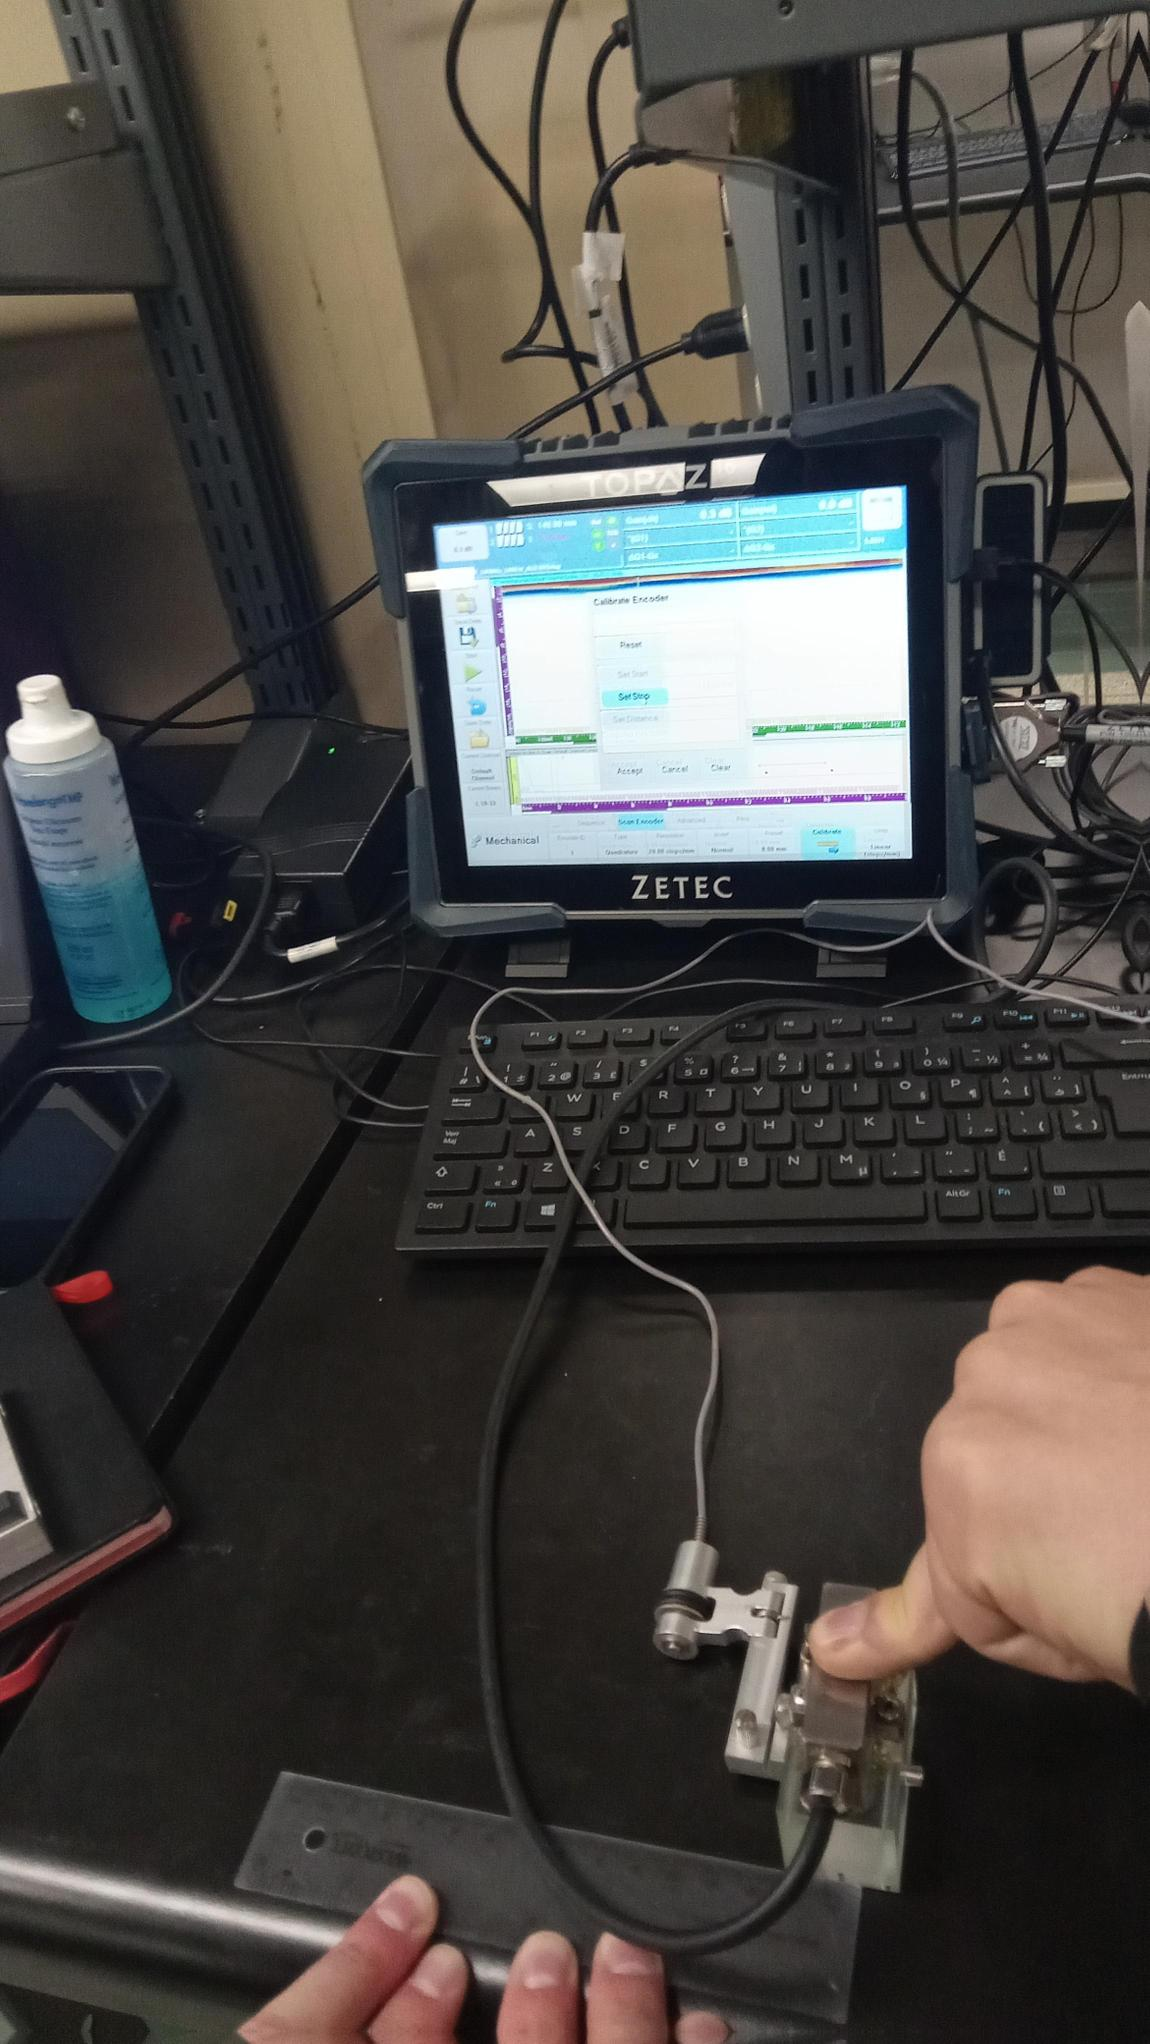
\includegraphics[height=9cm]{../../figures/Photos_Lab/Methode4.jpg}
\caption{Calibration de l'encodeur.}
\label{fig:methode-calibration-encodeur}
\end{figure}

\subsubsection*{\'Etape 6: sauvegarder la configuration}

Dans le menu File, appuyer sur Save Setup et donner un nom propre \`a l'\'equipe, pour ne pas \'ecraser la configuration du laboratoire ni celle d'une autre \'equipe.

\subsection{Calibration}
\label{sec:calibration}

La calibration fait en sorte que la profondeur et l'amplitude affich\'ees soient correctes pour les 49 faisceaux, et non seulement pour un seul. Sans calibration, deux faisceaux voisins peuvent afficher une profondeur ou une amplitude l\'eg\`erement diff\'erentes pour un m\^eme d\'efaut, parce que leur trajet dans le sabot et la r\'eponse de leurs \'el\'ements ne sont pas rigoureusement identiques. La calibration doit \^etre refaite \`a chaque s\'eance, et apr\`es tout changement de sonde, de sabot ou de loi focale.

Trois calibrations sont faites, dans cet ordre: la vitesse, le d\'elai de sabot, puis la sensibilit\'e. Toutes utilisent comme r\'eflecteur l'\'echo de fond d'un bloc d'aluminium \`a faces parall\`eles dont l'\'epaisseur $e$ a \'et\'e mesur\'ee au pied \`a coulisse, et dont la surface est plus grande que le sabot ($51 \times 28$~mm). Avec un sabot droit, tous les faisceaux voient l'\'echo de fond en m\^eme temps: il n'est donc pas n\'ecessaire de d\'eplacer la sonde pendant la calibration, il suffit de la tenir immobile avec une pression constante.

\subsubsection*{Pr\'eparation}

\begin{enumerate}
  \item Mettre du couplant sur le bloc et y poser la sonde, bien \`a plat.
  \item Ajuster le gain pour que l'\'echo de fond atteigne environ 80~\% de l'\'ecran sans saturer.
  \item Choisir le menu Calibration. La mise en page de l'\'ecran change pour la vue de calibration: la vue de tous les faisceaux en haut, le A-scan du faisceau choisi, et une courbe qui donne, pour chaque faisceau, la position ou l'amplitude maximale du r\'eflecteur.
\end{enumerate}

Les param\`etres du r\'eflecteur communs aux trois calibrations sont donn\'es au Tableau~\ref{tab:reflecteur}.

\begin{table}[H]
\centering
\caption{Param\`etres du r\'eflecteur communs aux trois calibrations (sous-menu Reflector).}
\label{tab:reflecteur}
\begin{tabular}{llp{6.5cm}}
\toprule
Param\`etre & Valeur & Remarque \\
\midrule
Reflector Type & Depth & le r\'eflecteur est \`a la m\^eme profondeur pour tous les faisceaux \\
Detection Mode & Maximum Amplitude & demand\'e pour la vitesse seulement \\
Detection Threshold & 20~\% & seuil de la porte de d\'etection \\
Diameter & 0~mm & si demand\'e, \'echo de fond et non un trou \\
Start & $e - 5$~mm & d\'ebut de la zone de recherche \\
Range & 10~mm & largeur de la zone de recherche \\
\bottomrule
\end{tabular}
\end{table}

\attention{Quand on calibre sur un bloc d'une autre \'epaisseur que celle de la configuration charg\'ee, il faut mettre \`a jour la cible (Target) et la zone de recherche (Start et Range) de chaque r\'eflecteur pour la nouvelle \'epaisseur $e$: Reflector~1 \`a $e$ et Reflector~2 \`a $2e$. Sinon, la zone de recherche peut attraper le mauvais \'echo, par exemple le deuxi\`eme \'echo de fond, et le d\'elai de sabot calcul\'e est faux. Si la pi\`ece est d'un autre alliage, il faut aussi refaire les trois calibrations sur ce bloc.}

\begin{figure}[H]
\centering
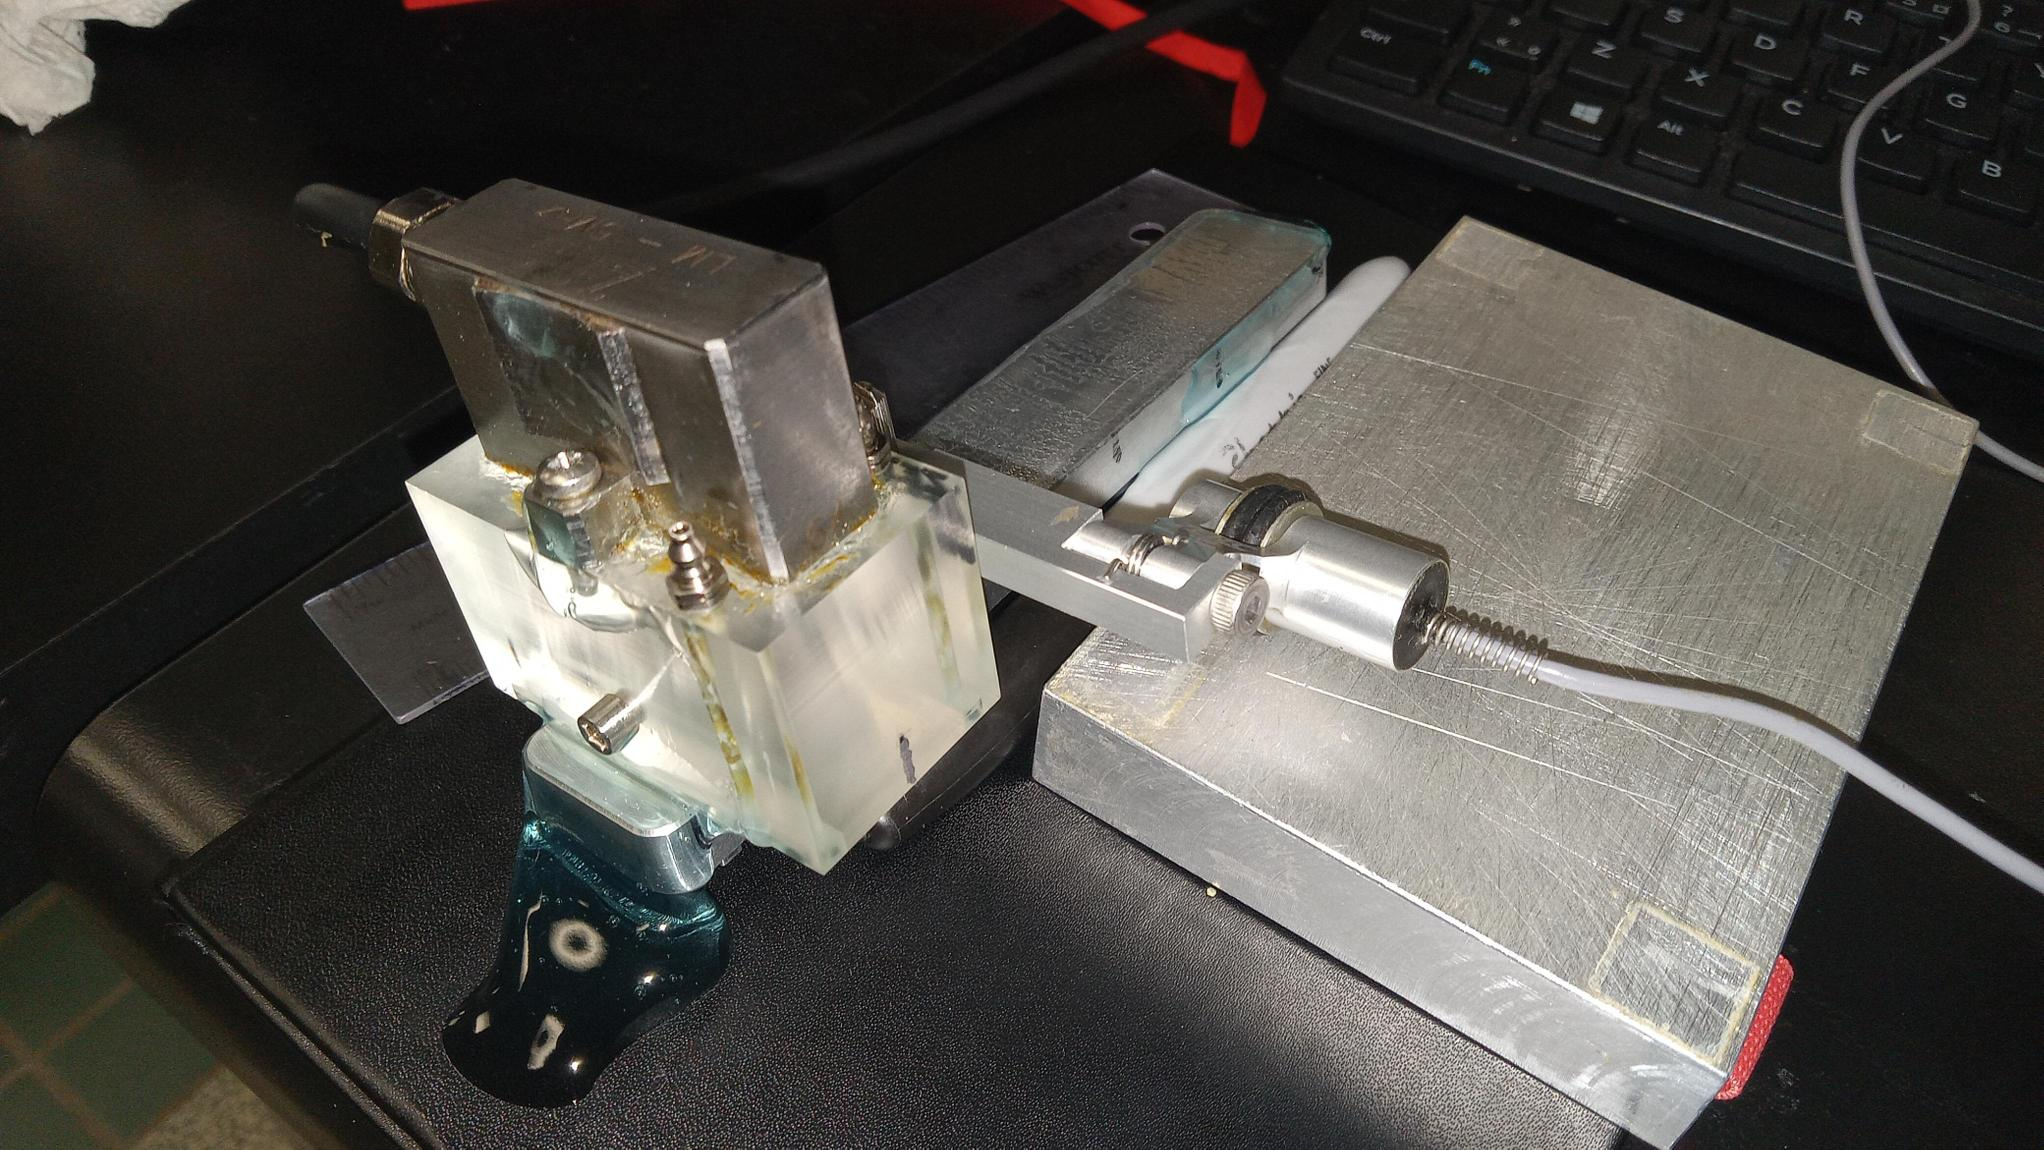
\includegraphics[width=10cm]{../../figures/Photos_Lab/PageTitreProtocole1.jpg}
\caption{Montage pour une calibration.}
\label{fig:montage-calibration}
\end{figure}

\subsubsection*{Calibration de la vitesse}

Cette calibration fixe la vitesse du son qui sert \`a convertir le temps de vol en profondeur. Elle demande deux r\'eflecteurs \`a des profondeurs diff\'erentes: le premier \'echo de fond, \`a la profondeur $e$, et le deuxi\`eme \'echo de fond, qui appara\^it \`a la profondeur $2e$ apr\`es un aller-retour de plus dans le bloc.

\begin{enumerate}
  \item Dans le menu Calibration, choisir Velocity.
  \item Dans le sous-menu Reflector~1, entrer les param\`etres du Tableau~\ref{tab:reflecteur} avec Target~$= e$.
  \item Dans le sous-menu Reflector~2, entrer les m\^emes param\`etres avec Target~$= 2e$ et Start~$= 2e - 5$~mm.
  \item Dans le sous-menu Calibrate, choisir comme Current Beam un faisceau du centre de la sonde, par exemple le faisceau~25.
  \item Appuyer sur Clear Envelope, attendre une ou deux secondes sans bouger la sonde, puis appuyer sur Compute~1.
  \item Appuyer sur Compute~2. L'appareil calcule la vitesse qui place les deux \'echos \`a leur profondeur cible.
  \item V\'erifier que la vitesse obtenue est proche de 6320~m/s (\`a quelques pour cent pr\`es), puis appuyer sur Accept.
\end{enumerate}

Une vitesse tr\`es diff\'erente indique en g\'en\'eral une erreur dans les cibles (\'epaisseur mal mesur\'ee, ou deuxi\`eme \'echo en dehors de la zone de recherche).

\subsubsection*{Calibration du d\'elai de sabot}

Cette calibration corrige, pour chaque faisceau, le d\'elai propre \`a son trajet dans le sabot, pour qu'un m\^eme r\'eflecteur apparaisse \`a la m\^eme profondeur peu importe le faisceau.

\begin{enumerate}
  \item Dans le menu Calibration, choisir Wedge Delay.
  \item Dans le sous-menu Reflector, entrer les param\`etres du Tableau~\ref{tab:reflecteur} avec Target~$= e$. Laisser la tol\'erance \`a sa valeur par d\'efaut.
  \item Dans le sous-menu Calibrate, appuyer sur Clear Envelope, attendre une ou deux secondes sans bouger la sonde, puis appuyer sur Compute.
  \item Pour v\'erifier le r\'esultat, appuyer de nouveau sur Clear Envelope et attendre une ou deux secondes. La courbe rouge de la vue de calibration doit alors \^etre plate \`a la profondeur $e$ pour les 49 faisceaux. Appuyer sur Accept.
\end{enumerate}

\subsubsection*{Calibration de la sensibilit\'e}

Cette calibration ajuste le gain de chaque faisceau pour qu'un m\^eme r\'eflecteur donne la m\^eme amplitude peu importe le faisceau.

\begin{enumerate}
  \item Dans le menu Calibration, choisir Sensitivity.
  \item Dans le sous-menu Reflector, entrer les param\`etres du Tableau~\ref{tab:reflecteur} avec Target~$= 80$~\% et Tolerance~$= 5$~\%.
  \item Dans le sous-menu Calibrate, appuyer sur Sector et s\'electionner tous les faisceaux (1 \`a 49).
  \item Appuyer sur Clear Envelope, attendre une ou deux secondes sans bouger la sonde, puis appuyer sur Compute.
  \item Pour v\'erifier le r\'esultat, appuyer de nouveau sur Clear Envelope et attendre une ou deux secondes. La courbe rouge doit alors \^etre plate \`a 80~\% pour tous les faisceaux, \`a l'int\'erieur de la tol\'erance. Appuyer sur Accept.
\end{enumerate}

Une fois les trois calibrations accept\'ees, les indicateurs V (vitesse), \textmu s (d\'elai de sabot) et dB (sensibilit\'e) de la zone d'\'etat doivent \^etre verts (Figure~\ref{fig:indicateurs}). Un indicateur gris signifie que la calibration n'a pas \'et\'e faite, et un indicateur jaune qu'au moins un faisceau n'a pas \'et\'e calibr\'e.

\begin{figure}[H]
\centering
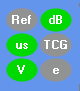
\includegraphics[width=4.5cm]{../../figures/Photos_Lab/IndicateurCalibration.png}
\caption{Indicateurs de calibration V, \textmu s et dB dans la zone d'\'etat.}
\label{fig:indicateurs}
\end{figure}

La correction de gain en fonction du temps (TCG) permet en plus de compenser l'att\'enuation avec la profondeur, pour qu'un m\^eme r\'eflecteur donne la m\^eme amplitude peu importe sa profondeur. Elle n'est pas utilis\'ee dans les manipulations propos\'ees ici.

\subsubsection*{Sauvegarder la configuration calibr\'ee}

V\'erifier que les indicateurs V, \textmu s et dB sont verts, puis refaire File, Save Setup avant toute acquisition. La sauvegarde de l'\'etape~6 de la Section~\ref{sec:configuration} a \'et\'e faite avant la calibration, donc elle ne contient pas les calibrations.

\subsection{Mesures et acquisition}
\label{sec:mesure}

\subsubsection*{Lire l'\'ecran}

En balayage lin\'eaire, la vue principale (appel\'ee VC sectorial scan dans UltraVision Touch) prend la forme d'une image rectangulaire: l'axe horizontal correspond aux 49 faisceaux c\^ote \`a c\^ote le long de la sonde, et l'axe vertical \`a la profondeur. La couleur donne l'amplitude de l'\'echo. Le A-scan affich\'e \`a c\^ot\'e est celui du faisceau choisi avec le curseur de loi (ligne noire dans la vue principale), qu'on d\'eplace avec le doigt.

\subsubsection*{Pi\`eges d'interpr\'etation}

\begin{itemize}
  \item Zone morte: l'\'echo d'interface sabot/pi\`ece et sa tra\^ine occupent environ les 2 premiers mm sous la surface. Un d\'efaut \`a cette profondeur est difficile \`a voir.
  \item \'Echos multiples: un r\'eflecteur plan \`a la profondeur $d$ produit aussi des \'echos \`a $2d$ et $3d$, apr\`es un ou deux allers-retours de plus. Ce ne sont pas des d\'efauts suppl\'ementaires.
  \item Les indicateurs E (v\'erification des \'el\'ements), Ref (gain de r\'ef\'erence) et TCG peuvent rester gris. Ils ne sont pas utilis\'es dans ces manipulations.
\end{itemize}

\subsubsection*{Mesurer une profondeur et une amplitude}

\begin{enumerate}
  \item Dans le menu UT Settings, sous-menu Gates, choisir Gate~1 et r\'egler State \`a On, Trigger \`a Crossing et Threshold \`a 25~\%.
  \item R\'egler Start et Range, dans le m\^eme sous-menu, pour que la porte (le trait horizontal sur le A-scan) couvre l'\'echo \`a mesurer, et seulement lui.
  \item Appuyer dans la zone des champs d'information (en haut de l'\'ecran) et choisir les champs D(G1), qui donne la profondeur de l'\'echo dans la porte, et \%(G1), qui donne son amplitude en pourcentage de l'\'ecran. S'ils ne font pas partie du groupe affich\'e, les ajouter avec Define Custom.
\end{enumerate}

\subsubsection*{Enregistrer les donn\'ees}

\begin{enumerate}
  \item Choisir le menu Inspection et r\'egler Action On Start \`a None (\`a Reset Encoder avec un encodeur, voir l'\'etape~5 de la Section~\ref{sec:configuration}).
  \item Appuyer sur Start. L'appareil enregistre les donn\'ees.
  \item Appuyer sur Stop, le gros bouton rouge \`a c\^ot\'e de Start. Dans la fen\^etre Save Data, entrer un nom de fichier et appuyer sur Accept. Le fichier .UVData est enregistr\'e dans le dossier Data.
  \item Pour garder une image de l'\'ecran (utile pour le rapport), choisir le menu Tools et appuyer sur Save Screen. L'image .PNG est enregistr\'ee dans le dossier Screens.
\end{enumerate}

Les fichiers peuvent ensuite \^etre copi\'es sur une cl\'e USB branch\'ee sur le panneau lat\'eral droit. Dans le Topaz, le fichier enregistr\'e se trouve dans le dossier Data, sous le nom donn\'e \`a l'enregistrement.

\begin{itemize}
  \item On peut aussi enregistrer directement sur la cl\'e USB: menu File, Other, Naming Option, Directory, puis choisir la cl\'e.
  \item Sinon, copier les fichiers avec le menu Tools, File Manager, depuis le dossier Data.
  \item Le fichier .UVExtension cr\'e\'e \`a c\^ot\'e du .UVData ne contient presque rien d'utile. C'est le .UVData qu'il faut garder.
\end{itemize}

\subsection{Arr\^et et entretien}

Fermer le fichier de donn\'ees avant d'\'eteindre, puis \'eteindre l'appareil proprement avec le bouton marche/arr\^et. Nettoyer le couplant sur le sabot, sur la sonde et sur le bloc. Remettre le capot de protection du connecteur de la sonde, puis recharger la batterie.

\section{Manipulations}
\label{sec:manipulations}

\subsection{Reprise des manipulations classiques avec le Topaz}

Les manipulations d\'ecrites \`a la section~3 du document Ultrasons, soit la mesure d'une \'epaisseur, la r\'eflexion sur une surface courb\'ee, la d\'etection d'une cavit\'e et la mesure de l'att\'enuation, peuvent toutes \^etre refaites avec le Topaz, avec la configuration et la calibration des Sections~\ref{sec:configuration} et~\ref{sec:calibration}.

Pour travailler avec un seul faisceau, comme avec une sonde \`a un seul \'el\'ement, placer le curseur de loi sur un faisceau du centre de la sonde (par exemple le faisceau~25, qui utilise les \'el\'ements 25 \`a 40). L'\'epaisseur se lit directement avec le champ D(G1) en pla\c cant la porte sur l'\'echo de fond (Section~\ref{sec:mesure}). Pour la mesure de l'att\'enuation, l'amplitude se lit avec \%(G1). Le gain doit alors rester le m\^eme pour tous les \'echantillons compar\'es.

\subsection{Balayage lin\'eaire d'un d\'efaut simul\'e}
\label{sec:manip-lineaire}

Cette manipulation utilise le balayage lin\'eaire d\'ecrit \`a la Section~\ref{sec:theorie}. La sonde reste immobile, et c'est l'ouverture active qui se d\'eplace le long du r\'eseau.

\subsubsection*{Montage et mesure}

\begin{enumerate}
  \item Configurer l'appareil avec les valeurs de la Section~\ref{sec:configuration} et le calibrer comme d\'ecrit \`a la Section~\ref{sec:calibration}.
  \item Mettre du couplant sur le bloc contenant le d\'efaut simul\'e fourni par le laboratoire, et poser la sonde de fa\c con \`a ce que le d\'efaut se trouve environ sous le milieu de la sonde. Les centres des 49 faisceaux couvrent une longueur de $48 \times 0{,}6 = 28{,}8$~mm.
  \item Sans bouger la sonde, rep\'erer dans la vue principale les faisceaux qui montrent l'\'echo du d\'efaut, entre la surface et l'\'echo de fond.
  \item Avec le curseur de loi, chercher le faisceau $n$ pour lequel l'\'echo du d\'efaut est le plus fort. Placer la porte sur cet \'echo et noter sa profondeur D(G1) et son amplitude \%(G1).
  \item Enregistrer les donn\'ees et une image de l'\'ecran (Section~\ref{sec:mesure}).
\end{enumerate}

Le faisceau $n$ utilise les \'el\'ements $n$ \`a $n+15$. Le centre de son ouverture se trouve donc \`a une distance
\begin{equation}
x_n = \left(n + 6{,}5\right) p
\label{eq:position}
\end{equation}
du centre du premier \'el\'ement, o\`u $p = 0{,}6$~mm est le pas de la sonde. Cette relation donne la position du d\'efaut le long de la sonde, et D(G1) donne sa profondeur.

\begin{figure}[H]
\centering
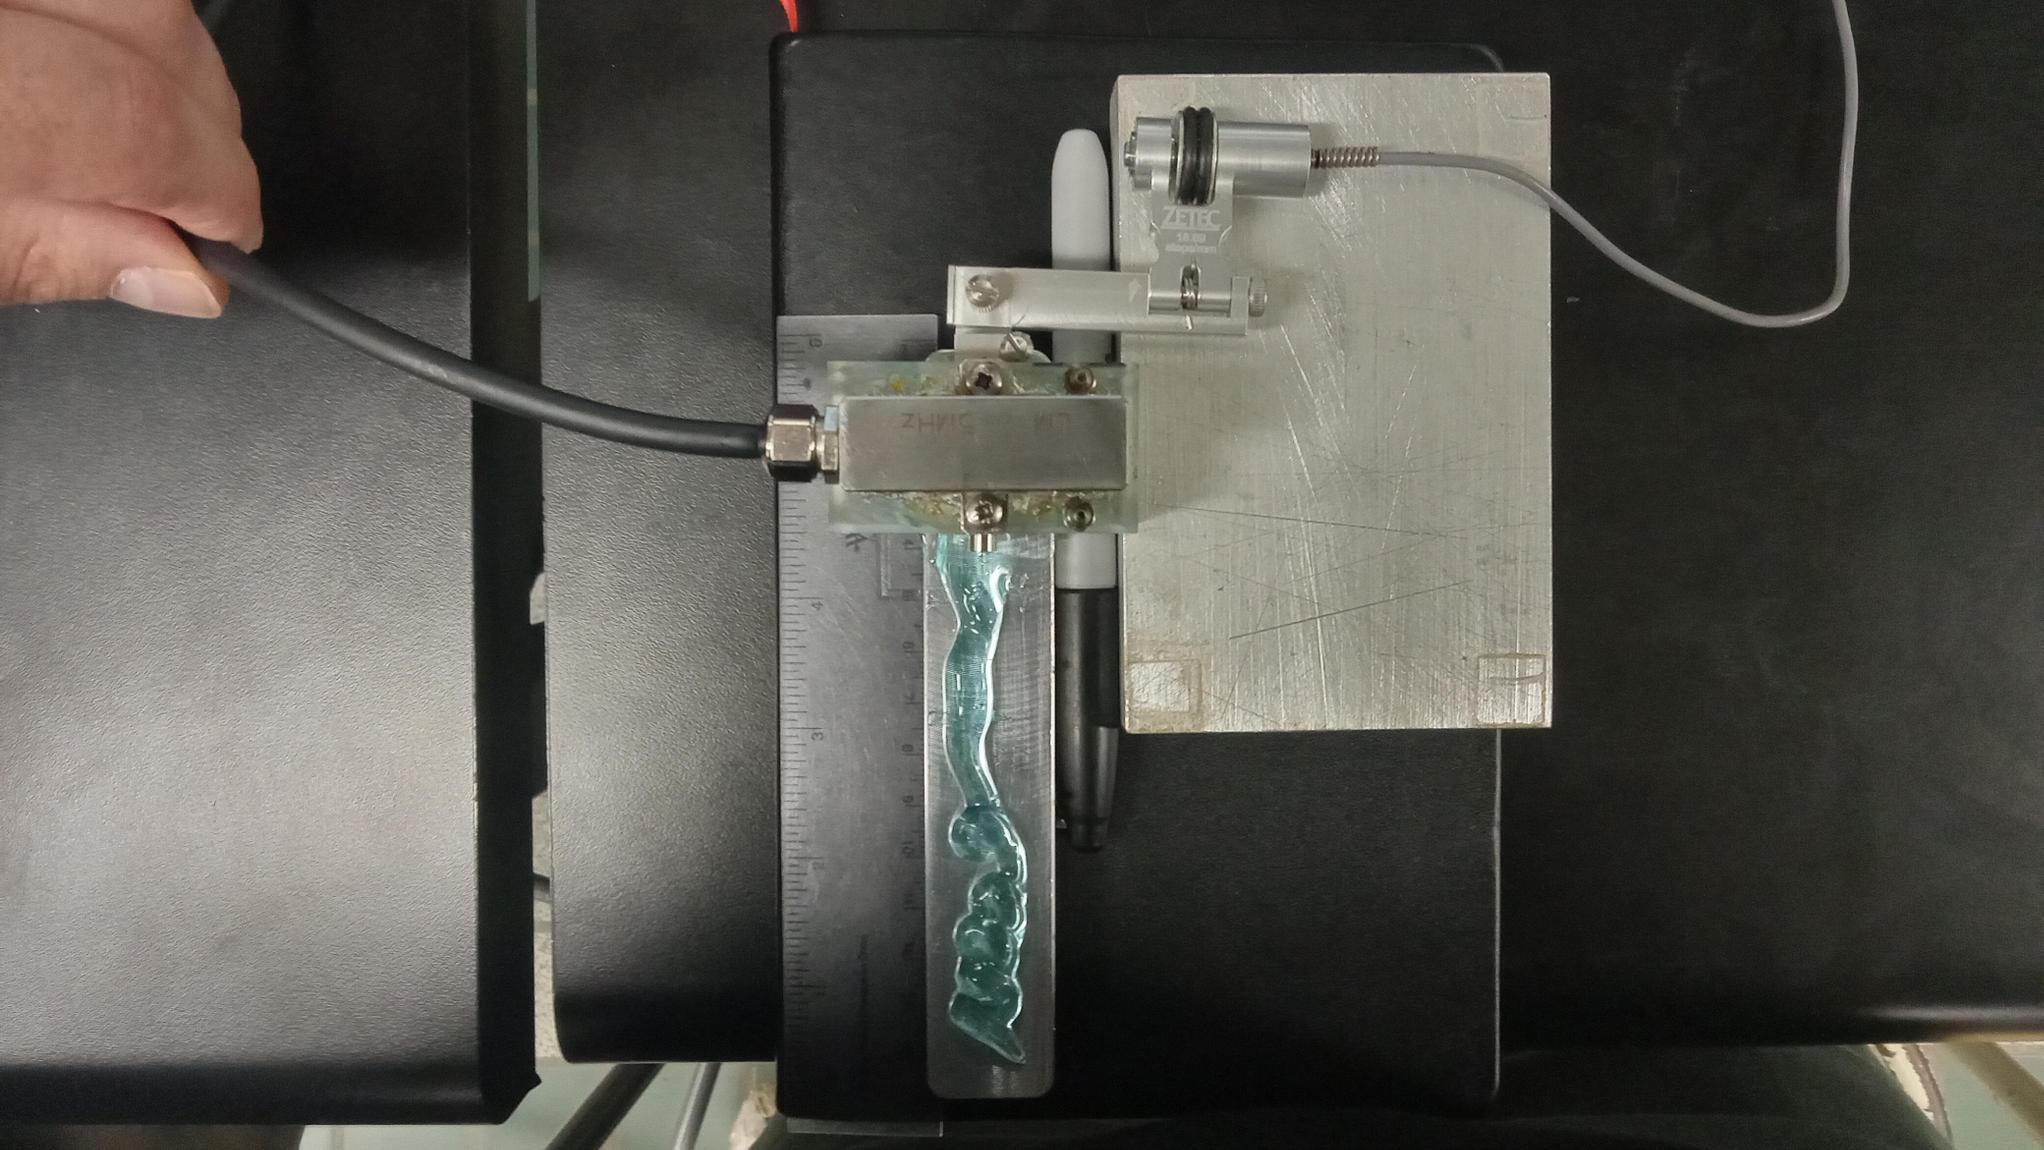
\includegraphics[width=10cm]{../../figures/Photos_Lab/Methode2.jpg}
\caption{Montage pour le balayage lin\'eaire d'un d\'efaut simul\'e.}
\label{fig:montage-manip}
\end{figure}

\subsection{Balayage avec d\'eplacement de la sonde (optionnel)}
\label{sec:manip-deplacement}

Cette manipulation reprend le bloc contenant le d\'efaut simul\'e, mais la sonde est d\'eplac\'ee \`a la main. Les A-scans enregistr\'es forment alors un volume, qui est analys\'e \`a la Section~\ref{sec:reconstruction}.

\subsubsection*{Montage et mesure}

\begin{enumerate}
  \item Configurer l'appareil et le calibrer (Sections~\ref{sec:configuration} et~\ref{sec:calibration}), puis sauvegarder la configuration calibr\'ee.
  \item R\'egler l'\'etape~5 de la Section~\ref{sec:configuration}: Sequence Type \`a One Line, Encoder ID \`a Clock, Acquisition Rate \`a 20~Hz, Scan Start \`a 0, Scan Stop assez grand pour tout le passage (par exemple 150~mm) et une r\'esolution de scan de 0,25~mm. Activer l'enregistrement des A-scans complets.
  \item Si un encodeur est utilis\'e, le brancher au Topaz et utiliser les r\'eglages de la variante avec encodeur de l'\'etape~5 (Section~\ref{sec:configuration}) au lieu de Clock. Les rep\`eres et la vitesse vis\'ee des \'etapes suivantes ne servent alors plus, mais il ne faut pas d\'eplacer la sonde trop rapidement.
  \item Coller des rep\`eres de ruban adh\'esif tous les 10~mm le long du bloc contenant le d\'efaut simul\'e, dans la direction perpendiculaire au r\'eseau de la sonde.
  \item Poser la sonde avec du couplant au d\'ebut du parcours, appuyer sur Start, puis la d\'eplacer \`a la main \`a vitesse constante (5~mm/s, soit un rep\`ere toutes les 2~s).
  \item Appuyer sur Stop d\`es la fin du d\'eplacement, puis enregistrer les donn\'ees et une image de l'\'ecran (Section~\ref{sec:mesure}).
  \item Analyser les donn\'ees en vue de dessus et en 3D (Section~\ref{sec:reconstruction}).
\end{enumerate}

\section{Reconstruction 3D \`a partir des fichiers .UVData}
\label{sec:reconstruction}

\subsection{Principe}

Une acquisition contient un A-scan complet pour chaque position de balayage et chaque faisceau. Empil\'es, ces A-scans forment un volume dont les trois axes sont la position de balayage, la position le long de la sonde et la profondeur. Un balayage lin\'eaire avec la sonde immobile (Section~\ref{sec:manip-lineaire}) ne donne qu'une seule tranche de ce volume. Pour obtenir un volume, il faut d\'eplacer la sonde (Section~\ref{sec:manip-deplacement}) et enregistrer les A-scans complets (\'etape~5 de la Section~\ref{sec:configuration}).

\subsection{Pr\'eparation des donn\'ees}

Quatre corrections sont n\'ecessaires. Les deux premi\`eres ne concernent que les acquisitions \`a l'horloge.

\begin{itemize}
  \item Remettre en ordre le tampon circulaire, si le d\'ebut a \'et\'e r\'e\'ecrit.
  \item Fixer le pas de balayage \`a partir de la vitesse de d\'eplacement de la main. Le pas est $\Delta s = v / f$, o\`u $v$ est la vitesse de d\'eplacement et $f$ la fr\'equence d'acquisition.
  \item Recaler la vitesse du son sur l'\'epaisseur connue du bloc, si la calibration n'a pas \'et\'e appliqu\'ee.
  \item Placer le z\'ero de profondeur sur l'\'echo de surface.
\end{itemize}

Pour une acquisition \`a l'horloge, UltraVision Touch 3.8R11 contient l'outil Scan Axis Repositioning, dans le menu Analysis, qui permet de remettre \`a l'\'echelle l'axe de balayage. Avec un encodeur, ce n'est pas n\'ecessaire.

\subsection{Conversion en CSV}

Le script Python \texttt{uvdata\_vers\_csv.py} est un outil qui permet d'utiliser les fichiers propri\'etaires .UVData d'UltraVision. Il convertit un fichier .UVData en CSV, sans aucun traitement des donn\'ees: le CSV contient les valeurs brutes enregistr\'ees par le Topaz, avec une ligne par A-scan. Sans encodeur, la position est simplement le num\'ero du coup d'horloge.

Le script est disponible dans le d\'ep\^ot GitHub \url{https://github.com/LouisFelixBRODEUR/Topaz16_GPH_3000}, qui contient:
\begin{itemize}
  \item le dossier \texttt{Docs\_ULTRAVISION}, avec les manuels d'utilisation du Topaz et d'UltraVision Touch,
  \item l'outil de conversion en CSV, \texttt{uvdata\_vers\_csv.py},
  \item un exemple de balayage avec encodeur, \texttt{Example\_Data\_Encodeur.UVData},
  \item un exemple de balayage sans encodeur, \texttt{Example\_Data\_Sans\_Encodeur.UVData}.
\end{itemize}

\section{Bibliographie}

Zetec, Inc. \emph{TOPAZ User Manual}, r\'evision 10046055-R08.

Zetec, \emph{UltraVision Touch 3.8R11, Limitations and Remaining Anomalies}.

Voir aussi le document \emph{Ultrasons} de ce cours pour la th\'eorie de base de la propagation, de la r\'eflexion et de l'att\'enuation des ultrasons.

\end{document}
